\chapter{可換環論の基礎}\label{ch:ch02}

\begin{chapterlead}
第1章で見たように，代数幾何学では図形 $X$ をその上の多項式関数のなす環 $k[X]$ によって調べる．
本章では，そのために必要な可換環論の基礎をまとめる．
環と環準同型（2.1節，2.2節），イデアル（2.3節），素イデアルと極大イデアル（2.4節），剰余環（2.5節），
多項式環（2.6節），Noether性とHilbertの基底定理（2.7節）を順に扱う．
各概念について，それが幾何学的に何を意味するか（たとえば「極大イデアル $=$ 点」「素イデアル $=$ 既約な図形」
「剰余環 $=$ 図形上の関数環」）を常に意識しながら進む．
群・環・体の最も基本的な定義については付録Bも参照されたい．
\end{chapterlead}

%======================================================================
\section{環の定義と基本構造}
%======================================================================

\subsection{環の定義}

\begin{mydef}{環}{ch02-ring}
集合 $R$ に二つの演算，和 $+:R\times R\to R$ と積 $\cdot:R\times R\to R$ が与えられ，次を満たすとき，$(R,+,\cdot)$ を\textbf{環}という．
\begin{enumerate}
  \item $(R,+)$ はアーベル群である．すなわち和は結合的かつ可換で，零元 $0$ が存在し，各 $a$ に加法逆元 $-a$ が存在する．
  \item 積は結合的である：$(ab)c=a(bc)$．
  \item 分配法則：$a(b+c)=ab+ac$，$(a+b)c=ac+bc$．
  \item 積に関する単位元 $1$ が存在する：$1\cdot a=a\cdot1=a$．
\end{enumerate}
\end{mydef}

条件 (4) を課さない流儀もある（2.1.3小節）が，本ノートでは特に断らない限り環は単位元をもつものとする．
定義から次の基本的な性質が導かれる．

\begin{myprop}{環の基本性質}{ch02-ring-basic}
環 $R$ の任意の元 $a,b$ に対して，次が成り立つ．
\begin{enumerate}
  \item $0\cdot a=a\cdot0=0$．
  \item $(-a)b=a(-b)=-(ab)$，特に $(-1)a=-a$．
  \item $(-a)(-b)=ab$．
\end{enumerate}
\end{myprop}

\begin{proof}
(1) 分配法則より $0\cdot a=(0+0)a=0\cdot a+0\cdot a$．両辺に $-(0\cdot a)$ を加えて $0\cdot a=0$．$a\cdot 0=0$ も同様．
(2) $ab+(-a)b=(a+(-a))b=0\cdot b=0$ より $(-a)b=-(ab)$．もう一方も同様．
(3) (2)を二回用いて $(-a)(-b)=-(a(-b))=-(-(ab))=ab$．
\end{proof}

これらは「当たり前」に見えるが，すべて公理から導かれる性質であることが重要である．
抽象的な環（たとえば多項式を何かで割った環）においても，普段の計算規則が安心して使えることを保証している．

\subsection{可換環と非可換環}

すべての $a,b\in R$ について $ab=ba$ が成り立つ環を\textbf{可換環}という．

\begin{myex}{可換環と非可換環}{ch02-comm-noncomm}
(1) 整数環 $\Z$，有理数体 $\Q$，実数体 $\R$，複素数体 $\C$，多項式環 $k[x_1,\dots,x_n]$ は可換環である．

(2) 体 $k$ 上の $n\times n$ 行列全体 $M_n(k)$ は，行列の和と積で環をなすが，$n\ge2$ のとき可換ではない．
実際
\[
  \begin{pmatrix}0&1\\0&0\end{pmatrix}\begin{pmatrix}0&0\\1&0\end{pmatrix}=\begin{pmatrix}1&0\\0&0\end{pmatrix}
  \ne\begin{pmatrix}0&0\\0&1\end{pmatrix}=\begin{pmatrix}0&0\\1&0\end{pmatrix}\begin{pmatrix}0&1\\0&0\end{pmatrix}.
\]

(3) 四元数 $\mathbb H=\{a+bi+cj+dk\}$（$i^2=j^2=k^2=ijk=-1$）は，$ij=k=-ji$ であるから非可換である．
ただし $0$ でないすべての元が逆元をもつ（斜体）．
\end{myex}

\begin{physbox}[可換性と古典・量子]
量子力学の観測量の代数は非可換である．たとえば一自由度の正準交換関係 $[\hat x,\hat p]=i\hbar$ から生成される代数
（Weyl代数）は非可換環である．$\hbar\to0$ の古典極限で，この代数は相空間上の関数環 $\C[x,p]$ という可換環になる．
代数幾何学が扱うのはこの可換な側であり，可換環 $R$ を「ある空間上の関数環」とみなすことが本ノートの基本的な見方である．
なお，超対称理論で現れる Grassmann 数の代数（$\theta_i\theta_j=-\theta_j\theta_i$）は「超可換」と呼ばれる別の構造であり，
本ノートでは扱わない．
\end{physbox}

\textbf{以下，本ノートでは「環」といえば単位元をもつ可換環を意味する．}
非可換環を扱うときは，その都度明示する．

\subsection{単位元を持つ環}

単位元 $1$ は存在すれば一意である（$1,1'$ がともに単位元なら $1=1\cdot1'=1'$）．
単位元をもたない環の例として，偶数全体 $2\Z$ がある．これは和と積について閉じており，環の公理 (1)〜(3) を満たすが，単位元をもたない．
後で見るように，$2\Z$ は $\Z$ の\emph{イデアル}であり（2.3節），単位元をもたない「環」の多くはイデアルとして自然に理解される．

$1=0$ となる環は $\{0\}$ のみである（$a=1\cdot a=0\cdot a=0$）．これを\textbf{零環}という．
零環は幾何学的には「空集合上の関数環」に対応する．

\begin{mydef}{可逆元・整域・体}{ch02-unit-domain}
$R$ を環とする．
\begin{enumerate}
  \item $ab=1$ となる $b\in R$ が存在する $a$ を\textbf{可逆元}（単元）という．可逆元全体 $R^\times$ は積について群をなす．
  \item $a\ne0$ で，ある $b\ne0$ に対して $ab=0$ となる $a$ を\textbf{零因子}という．
  \item ある $m\ge1$ に対して $a^m=0$ となる $a$ を\textbf{冪零元}という．
  \item $R\ne0$ で，零因子をもたない環を\textbf{整域}という．
  \item $R\ne0$ で，$0$ 以外のすべての元が可逆である環を\textbf{体}という．
\end{enumerate}
\end{mydef}

体は整域である：$a\ne0$，$ab=0$ ならば $b=a^{-1}ab=0$．また $0$ でない冪零元は零因子である
（$a^m=0$ で $m$ を最小にとれば $a\cdot a^{m-1}=0$，$a^{m-1}\ne0$）．

\begin{myex}{$\Z/6\Z$ と $\Z/5\Z$}{ch02-zmod}
$\Z/6\Z=\{\bar0,\bar1,\dots,\bar5\}$ では $\bar2\cdot\bar3=\bar0$ であるから $\bar2,\bar3$ は零因子であり，整域ではない．
可逆元は $\bar1,\bar5$ のみである．一方 $\Z/5\Z$ では $0$ でないすべての元が可逆であり（$\bar2\cdot\bar3=\bar1$，$\bar4\cdot\bar4=\bar1$），体である．
一般に $\Z/n\Z$ が体であることと $n$ が素数であることは同値である（2.4節）．
$\Z/8\Z$ では $\bar2^3=\bar0$ であり，$\bar2$ は冪零元である．
\end{myex}

幾何学的に言えば，零因子は「図形が複数の部分からなる」ことを，冪零元は「図形が重複した構造をもつ」ことを反映している．
たとえば $k[x,y]/(xy)$（2本の座標軸の関数環）では $x\cdot y=0$ であり，$x$ は $y$ 軸上で，$y$ は $x$ 軸上で消えている．
これは2.5.3小節で詳しく見る．

\subsection{部分環}

\begin{mydef}{部分環}{ch02-subring}
環 $R$ の部分集合 $S$ が，$1\in S$ を含み，和・差・積について閉じているとき，$S$ を $R$ の\textbf{部分環}という．
\end{mydef}

部分環は，$R$ の演算を制限することでそれ自身環になる．$1\in S$ を要求することに注意する．
この条件のため，たとえば $2\Z$ は $\Z$ の部分環ではない．

\begin{myex}{部分環の例}{ch02-subring-ex}
(1) $\Z\subset\Q\subset\R\subset\C$ はそれぞれ部分環である．

(2) \textbf{Gauss整数環} $\Z[i]=\{a+bi\mid a,b\in\Z\}$ は $\C$ の部分環である．

(3) $k$ を体とし，$k[x]$ の部分集合
\[
  k[x^2,x^3]=\{a_0+a_2x^2+a_3x^3+a_4x^4+\cdots\}
\]
（$x$ の一次の項をもたない多項式全体）は部分環である．実際，$x$ の一次の項をもたない多項式同士の積も一次の項をもたない．
この環は尖点をもつ曲線 $y^2=x^3$ の座標環と同型である（2.2.5小節）．
「一次の項がない」という条件が，原点で曲線が尖っていることに対応している．

(4) $R$ の部分集合 $T$ に対し，$T$ を含む最小の部分環（$T$ を含む部分環すべての共通部分）を $T$ が\textbf{生成する部分環}という．
$R$ が $S$ を部分環として含み，$a_1,\dots,a_n\in R$ のとき，$S\cup\{a_1,\dots,a_n\}$ が生成する部分環を $S[a_1,\dots,a_n]$ と書く．
これは $a_1,\dots,a_n$ の $S$ 係数多項式として書ける元全体である．たとえば $\Z[\sqrt2]=\{a+b\sqrt2\mid a,b\in\Z\}$．
\end{myex}

\subsection{環の例}

本ノートで頻繁に用いる環の例をまとめておく．

\begin{enumerate}
  \item \textbf{整数環} $\Z$．最も基本的な整域であり，あらゆる環 $R$ に対して唯一の環準同型 $\Z\to R$ が存在する（2.2.1小節）．
  \item \textbf{剰余環} $\Z/n\Z$．$n$ が素数 $p$ のとき有限体 $\F_p$ になる．
  \item \textbf{多項式環} $R[x_1,\dots,x_n]$．代数幾何学の主役である（2.6節）．
  \item \textbf{関数環}．位相空間 $X$ 上の実数値連続関数全体 $C(X)$ は，各点ごとの和と積で可換環をなす．
        $X$ が2点以上からなるとき，$C(X)$ は一般に零因子をもつ（台が交わらない2つの関数の積は $0$）．
  \item \textbf{直積環} $R_1\times R_2$．成分ごとの演算で環をなし，単位元は $(1,1)$ である．
        $e_1=(1,0)$，$e_2=(0,1)$ は $e_i^2=e_i$，$e_1e_2=0$，$e_1+e_2=1$ を満たす（\textbf{冪等元}）．
        幾何学的には，直積環は2つの空間の\emph{非交和}上の関数環に対応し，冪等元は各連結成分上で $1$，他で $0$ の関数である．
  \item \textbf{双対数の環} $k[\varepsilon]=k[x]/(x^2)$．$\varepsilon^2=0$ を満たす元 $\varepsilon$ をもつ．
        $f(a+\varepsilon)=f(a)+f'(a)\varepsilon$ が成り立つことから，接ベクトルや無限小変形を代数的に扱う道具となる（第7章，第12章，第16章）．
  \item \textbf{形式的冪級数環} $k[[x]]$．無限和 $\sum_{i\ge0}a_ix^i$ 全体であり，定数項が $0$ でない元は可逆である
        （例：$(1-x)^{-1}=1+x+x^2+\cdots$）．原点の「無限小近傍」上の関数環とみなせる（第6章）．
  \item \textbf{二次整数環} $\Z[\sqrt{-5}]=\{a+b\sqrt{-5}\mid a,b\in\Z\}$．素因数分解の一意性が成り立たない例として2.6.4小節で用いる．
\end{enumerate}

\exprob{prob:ch02-1-1}
$\Z/12\Z$ の可逆元，零因子，冪零元をすべて求めよ．

\exprob{prob:ch02-1-2}
双対数の環 $k[\varepsilon]$（$\varepsilon^2=0$）において，多項式 $f\in k[x]$ と $a\in k$ に対し $f(a+b\varepsilon)=f(a)+bf'(a)\varepsilon$ が成り立つことを示せ．
また $a+b\varepsilon$ が可逆であるための必要十分条件を求めよ．

%======================================================================
\section{環準同型}
%======================================================================

\subsection{環準同型の定義}

\begin{mydef}{環準同型}{ch02-hom}
環 $R,S$ の間の写像 $\varphi:R\to S$ が，任意の $a,b\in R$ に対して
\[
  \varphi(a+b)=\varphi(a)+\varphi(b),\qquad \varphi(ab)=\varphi(a)\varphi(b),\qquad \varphi(1)=1
\]
を満たすとき，$\varphi$ を\textbf{環準同型}という．
\end{mydef}

加法についての準同型性から $\varphi(0)=0$，$\varphi(-a)=-\varphi(a)$ が従う．
条件 $\varphi(1)=1$ は積の準同型性からは従わない（零写像を除外するために必要である）ので，定義に含めている．

\begin{myex}{環準同型の例}{ch02-hom-ex}
(1) 自然な射影 $\Z\to\Z/n\Z$，$a\mapsto\bar a$．

(2) \textbf{代入準同型}．$a\in k^n$ に対して $\mathrm{ev}_a:k[x_1,\dots,x_n]\to k$，$f\mapsto f(a)$．
これは「関数 $f$ の点 $a$ での値をとる」写像であり，代数幾何学で最も基本的な準同型である．

(3) 複素共役 $\C\to\C$，$z\mapsto\bar z$．

(4) 部分環の包含写像 $S\hookrightarrow R$．

(5) 非例：$\Z\to\Z$，$a\mapsto2a$ は加法を保つが，$2(ab)\ne(2a)(2b)$ となりうるし，$1\mapsto2\ne1$ である．
\end{myex}

任意の環 $R$ に対して，環準同型 $\Z\to R$ はただ一つ存在する．実際 $\varphi(1)=1$ から，$n>0$ に対して
$\varphi(n)=1+\dots+1$（$n$ 個），$\varphi(-n)=-\varphi(n)$ と決まってしまう．
この準同型の核は $n\Z$（$n\ge0$）の形をしており（2.3.4小節），この $n$ を $R$ の\textbf{標数}という．
$\Q,\R,\C$ の標数は $0$，$\F_p$ の標数は $p$ である．整域の標数は $0$ か素数である．

\subsection{核と像}

\begin{mydef}{核と像}{ch02-ker-im}
環準同型 $\varphi:R\to S$ に対して，
\[
  \Ker\varphi=\{a\in R\mid\varphi(a)=0\},\qquad \Img\varphi=\{\varphi(a)\mid a\in R\}
\]
をそれぞれ $\varphi$ の\textbf{核}，\textbf{像}という．
\end{mydef}

\begin{myprop}{核と像の性質}{ch02-ker-im-prop}
$\varphi:R\to S$ を環準同型とする．
\begin{enumerate}
  \item $\Img\varphi$ は $S$ の部分環である．
  \item $\Ker\varphi$ は加法について閉じており，さらに任意の $r\in R$，$a\in\Ker\varphi$ に対して $ra\in\Ker\varphi$ を満たす．
\end{enumerate}
\end{myprop}

\begin{proof}
(1) $1=\varphi(1)\in\Img\varphi$．$\varphi(a)\pm\varphi(b)=\varphi(a\pm b)$，$\varphi(a)\varphi(b)=\varphi(ab)$ より閉じている．
(2) $a,b\in\Ker\varphi$ ならば $\varphi(a+b)=0$，$\varphi(-a)=0$．また $\varphi(ra)=\varphi(r)\varphi(a)=\varphi(r)\cdot0=0$．
\end{proof}

性質 (2) を満たす部分集合を\textbf{イデアル}と呼ぶ（2.3節）．つまり\emph{環準同型の核はイデアルである}．
核は一般に部分環ではないことに注意しよう（$\varphi\ne$ 零写像で $S\ne0$ なら $1\notin\Ker\varphi$）．

\begin{myex}{代入準同型の核}{ch02-ev-kernel}
$a\in k$ に対し $\mathrm{ev}_a:k[x]\to k$ の核は，$f(a)=0$ となる多項式全体である．
因数定理（2.6.1小節）より，これは $x-a$ の倍数全体 $(x-a)=\{(x-a)g\mid g\in k[x]\}$ に一致する．
同様に，$a=(a_1,\dots,a_n)\in k^n$ に対して
\[
  \Ker(\mathrm{ev}_a)=(x_1-a_1,\dots,x_n-a_n)
\]
が成り立つ（問\ref{prob:ch02-2-1}）．これは「点 $a$ で消える関数全体」であり，第1章で $\m_a$ と書いたものである．
\end{myex}

\subsection{単射・全射・同型}

\begin{myprop}{単射性の判定}{ch02-injective}
環準同型 $\varphi:R\to S$ が単射であるための必要十分条件は $\Ker\varphi=\{0\}$ である．
\end{myprop}

\begin{proof}
単射ならば $\varphi(a)=0=\varphi(0)$ から $a=0$．逆に $\Ker\varphi=0$ とし，$\varphi(a)=\varphi(b)$ とすれば $\varphi(a-b)=0$ より $a=b$．
\end{proof}

\begin{mydef}{同型}{ch02-iso}
環準同型 $\varphi:R\to S$ が全単射であるとき，$\varphi$ を\textbf{同型写像}といい，$R$ と $S$ は\textbf{同型}であるといって $R\cong S$ と書く．
\end{mydef}

全単射な環準同型の逆写像は自動的に環準同型になる：$\varphi(\varphi^{-1}(a)\varphi^{-1}(b))=ab$ より $\varphi^{-1}(ab)=\varphi^{-1}(a)\varphi^{-1}(b)$，和も同様．
同型な環は「元の名前の付け方が違うだけ」であり，環論的性質（整域であること，イデアルの構造など）をすべて共有する．

\begin{myex}{同型の例}{ch02-iso-ex}
(1) $\Z/6\Z\cong\Z/2\Z\times\Z/3\Z$，$\bar a\mapsto(a\bmod 2,\ a\bmod 3)$．これは中国剰余定理（2.3.5小節）の特別な場合である．

(2) 体からの環準同型 $\varphi:K\to S$（$S\ne0$）は常に単射である．実際 $a\ne0$ ならば $1=\varphi(a)\varphi(a^{-1})$ より $\varphi(a)\ne0$．

(3) $\Z[i]\cong\Z[x]/(x^2+1)$，$\R[x]/(x^2+1)\cong\C$（2.5節）．
\end{myex}

\subsection{環の同型定理}

イデアル $I\subset R$ に対して，剰余類 $a+I=\{a+x\mid x\in I\}$ 全体の集合 $R/I$ には
\[
  (a+I)+(b+I)=(a+b)+I,\qquad (a+I)(b+I)=ab+I
\]
によって環の構造が入る．これを\textbf{剰余環}という．演算が代表元の取り方によらないことの確認を含め，
剰余環の構成は2.5.1小節で詳しく述べる．ここでは同型定理を先に述べておく．
自然な射影 $\pi:R\to R/I$，$a\mapsto a+I$ は全射環準同型で，$\Ker\pi=I$ である．

\begin{mythm}{準同型定理（第一同型定理）}{ch02-first-iso}
$\varphi:R\to S$ を環準同型とする．このとき
\[
  \bar\varphi:R/\Ker\varphi\ \xrightarrow{\ \sim\ }\ \Img\varphi,\qquad a+\Ker\varphi\mapsto\varphi(a)
\]
は well-defined な環の同型写像である．特に $\varphi$ が全射ならば $R/\Ker\varphi\cong S$．
\end{mythm}

\begin{proof}
$I=\Ker\varphi$ とおく．$a+I=b+I$ ならば $a-b\in I$ なので $\varphi(a)=\varphi(b)$；よって $\bar\varphi$ は well-defined．
環準同型であることは $\varphi$ が準同型であることから直ちに従う．全射性は明らか．
$\bar\varphi(a+I)=0$ ならば $a\in I$ すなわち $a+I=0+I$ なので，$\Ker\bar\varphi=0$ であり単射．
\end{proof}

\[
\begin{tikzcd}
  R \arrow[r,"\varphi"] \arrow[d,"\pi"'] & S\\
  R/\Ker\varphi \arrow[r,"\bar\varphi","\sim"'] & \Img\varphi \arrow[u,hook]
\end{tikzcd}
\]

\begin{myex}{放物線の座標環}{ch02-parabola}
$\varphi:k[x,y]\to k[x]$ を $x\mapsto x$，$y\mapsto x^2$ で定まる準同型とする（$f(x,y)\mapsto f(x,x^2)$）．
$\varphi$ は全射である．核を求めよう．明らかに $y-x^2\in\Ker\varphi$ である．
任意の $f\in k[x,y]$ を $k[x][y]$ の元とみて，$y$ についての一次式 $y-x^2$（$y$ について最高次係数 $1$）で割り算すると
\[
  f(x,y)=(y-x^2)q(x,y)+r(x),\qquad r\in k[x]
\]
と書ける（$y$ に $x^2$ を代入した余りが $r(x)=f(x,x^2)$ である）．$f\in\Ker\varphi$ ならば $0=\varphi(f)=r(x)$ なので
$f=(y-x^2)q$ となる．よって $\Ker\varphi=(y-x^2)$ であり，準同型定理より
\[
  k[x,y]/(y-x^2)\cong k[x].
\]
これは第1章1.4.3小節で予告した「放物線は直線と同型」という主張の代数的な証明である．
\end{myex}

準同型定理に加えて，次の二つの同型定理と対応定理がよく用いられる．証明はいずれも準同型定理を適切な写像に適用すればよい．

\begin{mythm}{第二・第三同型定理}{ch02-iso-thms}
$R$ を環とする．
\begin{enumerate}
  \item $A\subset R$ を部分環，$I\subset R$ をイデアルとすると，$A+I=\{a+x\mid a\in A,\ x\in I\}$ は部分環，$A\cap I$ は $A$ のイデアルであり，
        \[
          A/(A\cap I)\cong(A+I)/I.
        \]
  \item $I\subset J$ を $R$ のイデアルとすると，$J/I=\{x+I\mid x\in J\}$ は $R/I$ のイデアルであり，
        \[
          (R/I)\big/(J/I)\cong R/J.
        \]
\end{enumerate}
\end{mythm}

\begin{proof}
(1) 合成 $A\hookrightarrow A+I\to(A+I)/I$ は全射で，核は $A\cap I$ である．準同型定理を適用すればよい．
(2) $R/I\to R/J$，$a+I\mapsto a+J$ は（$I\subset J$ より）well-defined な全射準同型で，核は $J/I$ である．準同型定理を適用すればよい．
\end{proof}

(2) は「$I$ で割ってから $J/I$ で割るのは，一度に $J$ で割るのと同じ」という意味である．
幾何学的には，$\Zero(J)\subset\Zero(I)$ であり，図形 $\Zero(I)$ の中で部分図形 $\Zero(J)$ を切り出すことに対応する．

\subsection{多項式環の環準同型}

多項式環からの環準同型は，変数の行き先だけで決まる．

\begin{myprop}{多項式環の普遍性}{ch02-poly-universal}
$R,S$ を環，$\psi:R\to S$ を環準同型，$s_1,\dots,s_n\in S$ とする．このとき，環準同型
$\Phi:R[x_1,\dots,x_n]\to S$ で，$\Phi|_R=\psi$ かつ $\Phi(x_i)=s_i$（$i=1,\dots,n$）を満たすものがただ一つ存在する．
\end{myprop}

\begin{proof}
存在：$\Phi\big(\sum c_\alpha x^\alpha\big)=\sum\psi(c_\alpha)s_1^{\alpha_1}\cdots s_n^{\alpha_n}$ と定めれば，$S$ の可換性より環準同型になる．
一意性：環準同型は和と積を保つので，$R$ の元と $x_i$ の行き先が決まれば，それらの多項式の行き先は上の式に決まってしまう．
\end{proof}

特に，$k$ 上の多項式環 $k[x_1,\dots,x_n]$ から $k$ を含む環 $A$ への $k$ 上の準同型（$k$ の元を動かさないもの，\textbf{$k$代数準同型}）は，
$x_i$ の行き先 $a_i\in A$ を任意に指定することで一意に定まる．$A=k$ のときが代入準同型 $\mathrm{ev}_a$ である．

\paragraph{多項式写像と引き戻し．}
多項式 $F_1,\dots,F_n\in k[x_1,\dots,x_m]$ によって写像 $F=(F_1,\dots,F_n):\A^m\to\A^n$ が定まる．
このとき，$\A^n$ 上の関数 $g(y_1,\dots,y_n)$ を $F$ で引き戻した $g\circ F$ は $\A^m$ 上の多項式関数であり，
\[
  F^*:k[y_1,\dots,y_n]\to k[x_1,\dots,x_m],\qquad y_j\mapsto F_j(x)
\]
という $k$ 代数準同型が得られる．写像の向きが逆になっていることに注意しよう．
「空間の間の写像」と「関数環の間の準同型」が\emph{逆向きに}対応するというのは，代数幾何学の基本原理の一つである（第5章，第10章）．

\begin{myex}{尖点曲線のパラメータ表示}{ch02-cusp}
写像 $\A^1\to\A^2$，$t\mapsto(t^2,t^3)$ の像は尖点曲線 $C=\Zero(y^2-x^3)$ に含まれる．対応する準同型
\[
  \varphi:k[x,y]\to k[t],\qquad x\mapsto t^2,\ y\mapsto t^3
\]
の核と像を求めよう．任意の $f\in k[x,y]$ を，$y$ について最高次係数 $1$ の二次式 $y^2-x^3$ で割ると
\[
  f=(y^2-x^3)q+a(x)+b(x)y\qquad(a,b\in k[x])
\]
と書ける．このとき $\varphi(f)=a(t^2)+b(t^2)t^3$ であり，$a(t^2)$ は $t$ の偶数次の項のみ，$b(t^2)t^3$ は奇数次の項のみからなる．
したがって $\varphi(f)=0$ ならば $a=b=0$ であり，$\Ker\varphi=(y^2-x^3)$ を得る．
また像は $t^2,t^3$ で生成される部分環 $k[t^2,t^3]$（例\ref{ex:ch02-subring-ex}(3)）である．準同型定理より
\[
  k[x,y]/(y^2-x^3)\cong k[t^2,t^3]\subsetneq k[t].
\]
放物線の場合（例\ref{ex:ch02-parabola}）と異なり，像が $k[t]$ 全体にならない（$t$ が像に入らない）ことが，
尖点曲線が $\A^1$ と同型でないこと（原点が特異点であること）の代数的な表れである（第7章）．
\end{myex}

\exprob{prob:ch02-2-1}
$a=(a_1,\dots,a_n)\in k^n$ に対し，代入準同型 $\mathrm{ev}_a:k[x_1,\dots,x_n]\to k$ の核が $(x_1-a_1,\dots,x_n-a_n)$ に等しいことを示せ．
（ヒント：$x_i=(x_i-a_i)+a_i$ と書いて $f$ を $x_i-a_i$ の多項式として展開せよ．）

\exprob{prob:ch02-2-2}
$\varphi:k[x,y]\to k[t]$，$x\mapsto t^2-1$，$y\mapsto t(t^2-1)$ の核が $(y^2-x^2(x+1))$ であることを示せ．

%======================================================================
\section{イデアル}
%======================================================================

\subsection{イデアルの定義}

\begin{mydef}{イデアル}{ch02-ideal}
環 $R$ の部分集合 $I$ が次を満たすとき，$I$ を $R$ の\textbf{イデアル}という．
\begin{enumerate}
  \item $0\in I$ であり，$a,b\in I$ ならば $a+b\in I$．
  \item $a\in I$，$r\in R$ ならば $ra\in I$．
\end{enumerate}
$I\ne R$ のとき，$I$ を\textbf{真のイデアル}という．
\end{mydef}

(2) で $r=-1$ とすれば $-a\in I$ となるので，イデアルは加法部分群である．
条件 (2) は「$I$ の元に何を掛けても $I$ から出ない」という\emph{吸収性}であり，これがイデアルの本質である．

\begin{myex}{イデアルの例}{ch02-ideal-ex}
(1) $\{0\}$ と $R$ 自身はイデアルである．

(2) $n\Z=\{nm\mid m\in\Z\}$ は $\Z$ のイデアルである．

(3) 環準同型の核はイデアルである（命題\ref{prop:ch02-ker-im-prop}）．特に $\Ker(\mathrm{ev}_a)=(x_1-a_1,\dots,x_n-a_n)$．

(4) $X\subset k^n$ を任意の部分集合とするとき，
\[
  \Ideal(X)=\{f\in k[x_1,\dots,x_n]\mid \text{すべての }a\in X\text{ に対し }f(a)=0\}
\]
はイデアルである．実際，$X$ 上で消える2つの関数の和も $X$ 上で消え，$X$ 上で消える関数に任意の関数を掛けても $X$ 上で消える．
これを $X$ の\textbf{消滅イデアル}といい，第4章で詳しく調べる．
\end{myex}

\begin{myprop}{可逆元を含むイデアル}{ch02-unit-ideal}
$I$ を環 $R$ のイデアルとする．$I$ が可逆元を含むならば $I=R$ である．
特に，$R$ が体であることと，$R$ のイデアルが $\{0\}$ と $R$ のみ（かつ $R\ne0$）であることは同値である．
\end{myprop}

\begin{proof}
$u\in I$ が可逆ならば，任意の $r\in R$ に対し $r=(ru^{-1})u\in I$．
後半：$R$ が体なら，$0$ でないイデアルは可逆元を含むので $R$ に等しい．
逆に，イデアルが $0$ と $R$ のみとすると，$a\ne0$ に対し $aR=\{ar\mid r\in R\}$ は $0$ でないイデアルなので $aR=R$；すなわち $ar=1$ となる $r$ が存在する．
\end{proof}

\subsection{部分環とイデアルの違い}

部分環とイデアルはどちらも「和について閉じた部分集合」であるが，その性格は大きく異なる．
\begin{itemize}
  \item 部分環は $1$ を含むことを要請する．イデアルが $1$ を含めば $R$ 全体になってしまうので，\emph{真のイデアルは部分環ではない}．
  \item 部分環は自分自身の元同士の積で閉じていればよいが，イデアルは $R$ の任意の元との積で閉じていなければならない．
        たとえば $\Z$ は $\Q$ の部分環であるが，$\frac12\cdot1\notin\Z$ なので $\Q$ のイデアルではない．
\end{itemize}
環準同型との関係で言えば，\emph{像}は部分環であり，\emph{核}はイデアルである．
幾何学的には次のような対比がある．

\begin{table}[H]
\centering
\begin{tabular}{lll}
\hline
 & 典型例 & 幾何学的意味 \\
\hline
イデアル $I\subset k[X]$ & $\Ideal(Y)$（$Y\subset X$）& 部分図形 $Y$ 上で消える関数全体 \\
剰余環 $k[X]/I$ & $k[Y]$ & 部分図形上の関数環（制限）\\
部分環 $A\subset k[X]$ & $k[x^2,x^3]\subset k[x]$ & 写像 $X\to Y$ による引き戻し \\
\hline
\end{tabular}
\end{table}

つまり，イデアルは「部分空間（閉部分集合）を切り出す」ものであり，部分環は「空間を写像で別の空間に送る（つぶす）」ことに対応する．
たとえば $k[t^2,t^3]\subset k[t]$ は，写像 $\A^1\to C=\Zero(y^2-x^3)$，$t\mapsto(t^2,t^3)$ による引き戻しの像である．

\subsection{生成イデアル}

\begin{mydef}{生成イデアル}{ch02-generated}
環 $R$ の部分集合 $S$ に対し，$S$ を含む最小のイデアルを $S$ が\textbf{生成するイデアル}といい $(S)$ と書く．具体的には
\[
  (S)=\Big\{\sum_{i=1}^m r_is_i\ \Big|\ m\ge0,\ r_i\in R,\ s_i\in S\Big\}
\]
である．$S=\{a_1,\dots,a_n\}$ のとき $(a_1,\dots,a_n)$ と書き，有限個の元で生成されるイデアルを\textbf{有限生成}という．
\end{mydef}

右辺が $S$ を含むイデアルであること，および $S$ を含む任意のイデアルが右辺の元をすべて含むことは定義から明らかである．
イデアル $I$ の生成系の取り方は一意ではない．たとえば $k[x,y]$ において
\[
  (x,\ y)=(x+y,\ x-y)\quad(\mathrm{char}\,k\ne2),\qquad (y-x^2,\ y-1)=(y-1,\ x^2-1)
\]
である．第1章で見たように，零点集合 $\Zero(S)$ は $S$ ではなく $(S)$ のみで決まる（命題\ref{prop:ch01-zero-ideal}）．

\begin{myex}{$\Z[x]$ のイデアル $(2,x)$}{ch02-2x}
$\Z[x]$ において $(2,x)=\{2f+xg\mid f,g\in\Z[x]\}$ は定数項が偶数である多項式全体である．
このイデアルは1個の元では生成されない．実際 $(2,x)=(h)$ とすると，$2\in(h)$ より $h$ は $2$ の約数，すなわち $\pm1,\pm2$ のいずれかである．
$h=\pm2$ ならば $x\in(2)$ となり矛盾．$h=\pm1$ ならば $1\in(2,x)$ となるが，$1$ の定数項は奇数なので矛盾．
同様の議論で，$k[x,y]$ のイデアル $(x,y)$ も1個の元では生成されないことが示せる（問\ref{prob:ch02-3-1}）．
\end{myex}

\subsection{主イデアル}

1個の元 $a$ で生成されるイデアル $(a)=aR=\{ra\mid r\in R\}$ を\textbf{主イデアル}という．
すべてのイデアルが主イデアルである整域を\textbf{単項イデアル整域}（PID）という．

\begin{mythm}{$\Z$ と $k[x]$ は単項イデアル整域}{ch02-pid}
$\Z$ および体 $k$ 上の一変数多項式環 $k[x]$ は単項イデアル整域である．
\end{mythm}

\begin{proof}
$k[x]$ の場合を示す（$\Z$ の場合も，次数の代わりに絶対値を用いて同様に示せる）．
$I\ne0$ をイデアルとし，$I\setminus\{0\}$ の元で次数が最小のもの $g$ をとる．任意の $f\in I$ を $g$ で割ると，
$f=qg+r$，$r=0$ または $\deg r<\deg g$ となる（割り算の原理，2.6.1小節）．$r=f-qg\in I$ であり，$g$ の次数の最小性から $r=0$．
よって $I=(g)$．
\end{proof}

整域 $R$ において $(a)=(b)$ となるのは，ある可逆元 $u$ によって $a=ub$ となるとき，かつそのときに限る
（$a=rb$，$b=sa$ とすると $a=rsa$ より $a=0$ または $rs=1$）．このとき $a,b$ は\textbf{同伴}であるという．
たとえば $k[x]$ の $0$ でないイデアルは，ただ一つのモニック多項式（最高次係数が $1$）で生成される．

$\Z$ や $k[x]$ では，イデアル全体が「数」や「多項式」と（同伴を除いて）一対一に対応するので，イデアルを考える利点は見えにくい．
しかし多変数の多項式環 $k[x_1,\dots,x_n]$（$n\ge2$）は単項イデアル整域ではなく（例\ref{ex:ch02-2x}の最後の注意），
「1つの方程式では書けない図形」（たとえば $\A^2$ の点，$\A^3$ の曲線）を扱うためにイデアルが本質的に必要になる．

\subsection{イデアルの和と積}

\begin{mydef}{イデアルの演算}{ch02-ideal-ops}
$I,J$ を環 $R$ のイデアルとする．
\[
  I+J=\{a+b\mid a\in I,\ b\in J\},\qquad IJ=\Big\{\sum_{i=1}^m a_ib_i\ \Big|\ a_i\in I,\ b_i\in J\Big\},\qquad I\cap J
\]
はいずれもイデアルであり，それぞれ\textbf{和}，\textbf{積}，\textbf{共通部分}という．
\end{mydef}

$I+J$ は $I\cup J$ が生成するイデアル，すなわち $I,J$ をともに含む最小のイデアルである．
積 $IJ$ は単なる積 $ab$ の集合ではなく，その有限和全体であることに注意する（積の集合は一般に和で閉じない）．
常に $IJ\subset I\cap J\subset I,J\subset I+J$ が成り立つ．
生成元で書けば $(a_1,\dots,a_m)+(b_1,\dots,b_n)=(a_1,\dots,a_m,b_1,\dots,b_n)$，$(a_1,\dots,a_m)(b_1,\dots,b_n)=(a_ib_j)_{i,j}$ である．

\begin{myex}{$\Z$ におけるイデアルの演算}{ch02-z-ops}
$\Z$ において
\[
  (m)+(n)=(\gcd(m,n)),\qquad (m)\cap(n)=(\mathrm{lcm}(m,n)),\qquad (m)(n)=(mn).
\]
たとえば $(4)+(6)=(2)$，$(4)\cap(6)=(12)$，$(4)(6)=(24)$．第1式は，$\gcd(m,n)=am+bn$ と書けるという Bézout の等式に他ならない．
\end{myex}

幾何学的には，これらの演算は次のように解釈される（第3章，第4章）．
\[
  \Zero(I+J)=\Zero(I)\cap\Zero(J),\qquad \Zero(IJ)=\Zero(I\cap J)=\Zero(I)\cup\Zero(J).
\]
すなわち\emph{イデアルの和は図形の共通部分に，積や共通部分は図形の和集合に}対応する．
たとえば $k[x,y]$ において
\[
  \begin{aligned}
  (x)+(y)&=(x,y) &&\leftrightarrow\ \text{原点}=\text{$y$軸}\cap\text{$x$軸},\\
  (x)\cap(y)&=(x)(y)=(xy) &&\leftrightarrow\ \text{両軸の和集合}.
  \end{aligned}
\]
ただし $IJ$ と $I\cap J$ は一般には異なる．たとえば $I=J=(x)$ のとき $IJ=(x^2)\ne(x)=I\cap J$ であり，
両者の零点集合は同じだが，$(x^2)$ は「$y$軸を2重に数えた」情報をもつ．

\begin{mythm}{中国剰余定理}{ch02-crt}
$R$ のイデアル $I,J$ が $I+J=R$ を満たす（\textbf{互いに素}である）ならば，$IJ=I\cap J$ であり，
\[
  R/(I\cap J)\ \cong\ R/I\times R/J,\qquad a+I\cap J\mapsto(a+I,\ a+J).
\]
\end{mythm}

\begin{proof}
$I+J=R$ より $e+f=1$ となる $e\in I$，$f\in J$ が存在する．
$x\in I\cap J$ ならば $x=xe+xf$ であり，$xe\in JI$，$xf\in IJ$ なので $x\in IJ$．よって $I\cap J=IJ$．
写像 $\varphi:R\to R/I\times R/J$，$a\mapsto(a+I,a+J)$ の核は $I\cap J$ である．
全射性：任意の $(a,b)$ に対し $x=af+be$ とおくと，$f\equiv1\pmod I$，$e\equiv0\pmod I$ より $x\equiv a\pmod I$，同様に $x\equiv b\pmod J$．
準同型定理より主張が従う．
\end{proof}

幾何学的には，$I+J=R$ は $\Zero(I)\cap\Zero(J)=\emptyset$（2つの図形が交わらない）ことに対応し，
このとき「非交和上の関数環は各成分上の関数環の直積である」というのが中国剰余定理の意味である．
たとえば $k[x]/(x(x-1))\cong k[x]/(x)\times k[x]/(x-1)\cong k\times k$ は，2点 $\{0,1\}$ 上の関数環である．

\subsection{イデアルの包含関係}

$\Z$ において $(a)\subset(b)$ であることは，$a\in(b)$，すなわち $b$ が $a$ を割り切ることと同値である．
「含む方が約数」であり，イデアルとして大きいほど生成元は「小さい」．たとえば $(12)\subset(6)\subset(3)\subset(1)$．
一般の環でも，$(a)\subset(b)\iff b\mid a$ が成り立つ．
したがってイデアルの包含関係は，整除関係を一般化したものとみなせる．「含むことは割ることである（to contain is to divide）」
という標語がある．

\begin{figure}[H]
\centering
\begin{tikzpicture}[scale=1.1,>=Stealth]
  \node (1) at (0,3) {$(1)=\Z$};
  \node (2) at (-1.2,2) {$(2)$};
  \node (3) at (1.2,2) {$(3)$};
  \node (4) at (-1.2,1) {$(4)$};
  \node (6) at (1.2,1) {$(6)$};
  \node (12) at (0,0) {$(12)$};
  \draw (12)--(4) (12)--(6) (4)--(2) (6)--(2) (6)--(3) (2)--(1) (3)--(1);
  \node[align=left,font=\small] at (5,1.5) {線分は下から上への包含 $\subset$ を表す．\\
     $(2),(3)$ は $(12)$ を含む極大イデアル．\\
     $\Z/12\Z$ のイデアルはこの6個と一対一に対応する．};
\end{tikzpicture}
\caption{$(12)$ を含む $\Z$ のイデアルの包含関係（Hasse図）}
\label{fig:ch02-hasse}
\end{figure}

幾何学との対応では，包含関係が逆転する：$I\subset J$ ならば $\Zero(I)\supset\Zero(J)$．
「方程式（イデアル）が増えれば解（図形）は小さくなる」のである．
たとえば $(y-x^2)\subset(y-x^2,\ y-1)$ に対して，放物線 $\supset$ 2点 $\{(\pm1,1)\}$ となる．
イデアルが大きいほど図形は小さく，最も大きい真のイデアル（極大イデアル）は最も小さい空でない図形，すなわち点に対応する．
これが次節の主題である．

\exprob{prob:ch02-3-1}
$k[x,y]$ のイデアル $(x,y)$ は単項イデアルでないことを示せ．

\exprob{prob:ch02-3-2}
$k[x]$（$\mathrm{char}\,k\ne2,3$ とする）において，$(x^2-1)+(x^2-3x+2)$，$(x^2-1)\cap(x^2-3x+2)$，$(x^2-1)(x^2-3x+2)$ をそれぞれ1つの元で生成されるイデアルとして表し，
対応する $\A^1$ の点集合（重複度に注意）を答えよ．

%======================================================================
\section{素イデアルと極大イデアル}
%======================================================================

\subsection{素イデアルの定義}

\begin{mydef}{素イデアル}{ch02-prime}
環 $R$ の真のイデアル $\p$ が，
\[
  ab\in\p\ \Longrightarrow\ a\in\p\ \text{または}\ b\in\p
\]
を満たすとき，$\p$ を\textbf{素イデアル}という．
\end{mydef}

これは素数の性質「$p\mid ab\Rightarrow p\mid a$ または $p\mid b$」の一般化である．実際，$\Z$ の素イデアルは
$(0)$ と $(p)$（$p$ は素数）のみである．$(6)$ は $2\cdot3\in(6)$ だが $2,3\notin(6)$ なので素イデアルでない．

\begin{myex}{多項式環の素イデアル}{ch02-prime-ex}
$k$ を体とする．
(1) $k[x,y]$ において $(x)$ は素イデアルである．実際 $k[x,y]/(x)\cong k[y]$ は整域である（2.4.4小節の判定法による）．
幾何学的には $(x)$ は $y$ 軸 $\Zero(x)$ に対応する．

(2) $(xy)$ は素イデアルでない．$x\cdot y\in(xy)$ だが $x,y\notin(xy)$．これは $\Zero(xy)$ が2本の直線に分かれることに対応する．

(3) $(x^2)$ も素イデアルでない．$x\cdot x\in(x^2)$ だが $x\notin(x^2)$．これは「重複」があることに対応する．

(4) $(x,y)$ は素イデアルである（$k[x,y]/(x,y)\cong k$ は体，とくに整域）．
\end{myex}

素イデアルは，幾何学的には\textbf{既約な}図形，すなわち「2つの真に小さい図形の和集合に分解できない図形」に対応する（第3章，第4章）．
$f\cdot g$ が図形 $X$ 上で消えるとき，$X$ が既約ならば $X$ は $\Zero(f)\cap X$ と $\Zero(g)\cap X$ のどちらか一方に含まれる，
すなわち $f$ または $g$ が $X$ 上で消える，という論理である．

素イデアルの定義は，イデアルについての形にも言い換えられる：
$\p$ が素イデアルで，イデアル $I,J$ が $IJ\subset\p$ を満たせば $I\subset\p$ または $J\subset\p$．
（$I\not\subset\p$ として $a\in I\setminus\p$ をとると，任意の $b\in J$ に対して $ab\in\p$ より $b\in\p$．）

\subsection{極大イデアルの定義}

\begin{mydef}{極大イデアル}{ch02-maximal}
環 $R$ の真のイデアル $\m$ が，包含関係について極大であるとき，すなわち
\[
  \m\subset I\subset R\ (I\text{ はイデアル})\ \Longrightarrow\ I=\m\ \text{または}\ I=R
\]
を満たすとき，$\m$ を\textbf{極大イデアル}という．
\end{mydef}

\begin{myex}{極大イデアルの例}{ch02-maximal-ex}
(1) $\Z$ の極大イデアルは $(p)$（$p$ は素数）である．$(0)$ は素イデアルだが $(0)\subsetneq(2)$ なので極大でない．

(2) $k[x]$ において，$a\in k$ に対し $(x-a)$ は極大イデアルである．$k[x]/(x-a)\cong k$ は体であるから（2.4.5小節）．

(3) $k[x_1,\dots,x_n]$ において，$a\in k^n$ に対し $\m_a=(x_1-a_1,\dots,x_n-a_n)$ は極大イデアルである．
これは代入準同型 $\mathrm{ev}_a$ の核であり，$k[x_1,\dots,x_n]/\m_a\cong k$ は体である．

(4) $\R[x]$ において $(x^2+1)$ は極大イデアルであるが，$\R$ の点には対応しない．$\R[x]/(x^2+1)\cong\C$ であり，
これは「共役な複素数の組 $\{\pm i\}$」に対応する．第1章で見た実数上の代数幾何の難しさが，ここに代数的に現れている．
\end{myex}

極大イデアルの存在は，一般には選択公理（Zornの補題）を用いて示される．

\begin{mythm}{極大イデアルの存在}{ch02-max-exist}
$R\ne0$ を環とし，$I$ を $R$ の真のイデアルとする．このとき $I$ を含む極大イデアルが存在する．
\end{mythm}

\begin{proof}
$I$ を含む真のイデアル全体の集合 $\Sigma$ を包含関係で順序付ける．$I\in\Sigma$ なので $\Sigma\ne\emptyset$．
$\{I_\lambda\}$ を $\Sigma$ の全順序部分集合（鎖）とすると，$J=\bigcup_\lambda I_\lambda$ はイデアルである
（$a\in I_\lambda$，$b\in I_\mu$ ならば，鎖であるからどちらか大きい方に $a,b$ がともに含まれる）．
また $1\notin I_\lambda$（すべての $\lambda$）より $1\notin J$ なので $J\in\Sigma$ は鎖の上界である．
Zornの補題より $\Sigma$ は極大元 $\m$ をもち，これが $I$ を含む極大イデアルである．
\end{proof}

\begin{note}
本ノートで主に扱う Noether 環（2.7節）では，Zornの補題を用いずに極大イデアルの存在を示すことができる
（真のイデアルの空でない族は極大元をもつ）．
\end{note}

\subsection{素イデアルと極大イデアルの関係}

\begin{myprop}{極大イデアルは素イデアル}{ch02-max-prime}
極大イデアルは素イデアルである．
\end{myprop}

\begin{proof}
$\m$ を極大イデアルとし，$ab\in\m$，$a\notin\m$ とする．$\m+(a)$ は $\m$ を真に含むイデアルなので $R$ に等しい．
よって $1=m+ra$（$m\in\m$，$r\in R$）と書ける．両辺に $b$ を掛けると $b=mb+rab\in\m$．
\end{proof}

逆は成り立たない：$\Z$ の $(0)$，$k[x,y]$ の $(x)$ は素イデアルだが極大でない．
幾何学的には，$(x)$ は $y$ 軸という1次元の既約図形に対応し，それはさらに点 $(0,b)$ に対応する極大イデアル $(x,y-b)$ に含まれる．
素イデアルの鎖
\[
  (0)\subsetneq(x)\subsetneq(x,y)
\]
は，図形の列「平面 $\supsetneq$ 直線 $\supsetneq$ 点」に対応する（図\ref{fig:ch02-chain}）．
このような鎖の長さで次元を定義するのが\textbf{Krull次元}である（第7章）．

\begin{figure}[H]
\centering
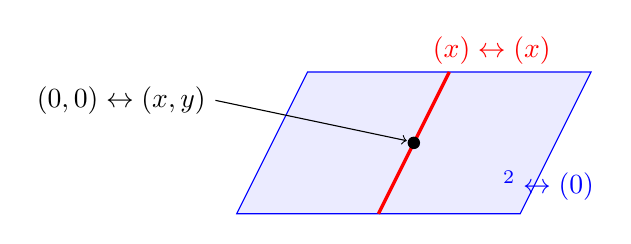
\begin{tikzpicture}[scale=0.9]
  \fill[blue!8] (0,0)--(4,0)--(5,2)--(1,2)--cycle;
  \draw[blue] (0,0)--(4,0)--(5,2)--(1,2)--cycle;
  \draw[very thick,red] (2,0)--(3,2);
  \fill (2.5,1) circle (2.5pt);
  \node[blue] at (4.4,0.4) {$\A^2\leftrightarrow(0)$};
  \node[red] at (3.6,2.3) {$\Zero(x)\leftrightarrow(x)$};
  \node[left] at (-0.3,1.6) {$(0,0)\leftrightarrow(x,y)$};
  \draw[->] (-0.3,1.6)--(2.4,1.03);
\end{tikzpicture}
\caption{素イデアルの鎖 $(0)\subsetneq(x)\subsetneq(x,y)$ と図形の列 $\A^2\supsetneq\text{直線}\supsetneq\text{点}$．包含の向きが逆転する．}
\label{fig:ch02-chain}
\end{figure}

単項イデアル整域では状況が単純である．

\begin{myprop}{PID の素イデアル}{ch02-pid-prime}
$R$ を単項イデアル整域とする．$0$ でない素イデアルは極大イデアルである．
\end{myprop}

\begin{proof}
$\p=(p)\ne0$ を素イデアルとし，$\p\subset(a)$ とする．$p=ab$ と書け，$p\mid a$ または $p\mid b$ である．
$p\mid a$ ならば $(a)=(p)$．$p\mid b$ ならば $b=pc$ と書け，$p=apc$ から（$R$ は整域で $p\ne0$）$ac=1$，すなわち $(a)=R$．
\end{proof}

したがって $\Z$ や $k[x]$ の素イデアルは，$(0)$ と極大イデアルのみである．
$\Z$ の素イデアル全体を図示すると図\ref{fig:ch02-specz}のようになる．
各素数 $p$ が「点」に対応し，$(0)$ は特定の点に対応しない特別な点（\textbf{生成点}）である．
このように素イデアル全体を空間とみなす考え方が，第12章のスキーム $\Spec R$ である．

\begin{figure}[H]
\centering
\begin{tikzpicture}
  \draw[thick] (0,0)--(9.5,0);
  \foreach \x/\p in {0.5/2,1.5/3,2.5/5,3.5/7,4.5/11,5.5/13,6.5/17}{
    \fill (\x,0) circle (2.5pt); \node[below] at (\x,-0.1) {$(\p)$};}
  \node at (7.6,0.25) {$\cdots$};
  \node[red] at (4.5,1) {$(0)$（生成点）};
  \draw[red,dashed,->] (4.5,0.75)--(4.5,0.1);
\end{tikzpicture}
\caption{$\Z$ の素イデアル全体の模式図．各素数 $p$ が閉点 $(p)$ に，$(0)$ が「直線全体に広がった」生成点に対応する．}
\label{fig:ch02-specz}
\end{figure}

\subsection{整域と素イデアル}

\begin{mythm}{素イデアルと整域}{ch02-prime-domain}
環 $R$ のイデアル $\p$ に対し，$\p$ が素イデアルであることと，剰余環 $R/\p$ が整域であることは同値である．
\end{mythm}

\begin{proof}
$R/\p\ne0\iff\p\ne R$．また $\bar a\bar b=\bar0$ in $R/\p$ $\iff ab\in\p$，$\bar a=\bar0\iff a\in\p$ である．
したがって「$R/\p$ に零因子がない」ことは「$ab\in\p\Rightarrow a\in\p$ または $b\in\p$」と同値である．
\end{proof}

特に，環 $R$ が整域であることと $(0)$ が素イデアルであることは同値である．
この定理は，素イデアルであるかどうかの判定によく使われる．たとえば
$k[x,y]/(y-x^2)\cong k[x]$ は整域なので $(y-x^2)$ は素イデアル（放物線は既約），
$k[x,y]/(xy)$ は $x\cdot y=0$ より整域でないので $(xy)$ は素イデアルでない．

\begin{myprop}{素イデアルの引き戻し}{ch02-prime-pullback}
$\varphi:R\to S$ を環準同型，$\q$ を $S$ の素イデアルとすると，$\varphi^{-1}(\q)$ は $R$ の素イデアルである．
\end{myprop}

\begin{proof}
$\varphi^{-1}(\q)$ がイデアルであることは容易．$\varphi(1)=1\notin\q$ より真のイデアル．
$ab\in\varphi^{-1}(\q)$ ならば $\varphi(a)\varphi(b)\in\q$ より $\varphi(a)\in\q$ または $\varphi(b)\in\q$．
（あるいは，$R/\varphi^{-1}(\q)$ が整域 $S/\q$ の部分環と同型であることからも従う．）
\end{proof}

これに対し，極大イデアルの引き戻しは極大とは限らない．包含 $\Z\hookrightarrow\Q$ において，$\Q$ の極大イデアル $(0)$ の引き戻しは
$\Z$ の $(0)$ であり，極大でない．この非対称性が，スキーム論で「点」として素イデアル全体を採用する理由の一つである（第12章）．
ただし，体 $k$ 上有限生成な $k$ 代数の間の $k$ 代数準同型については，極大イデアルの引き戻しは極大イデアルになる
（零点定理の帰結，第4章）．これが「多様体の射は点を点に写す」ことに対応する．

\subsection{体と極大イデアル}

\begin{mythm}{極大イデアルと体}{ch02-max-field}
環 $R$ のイデアル $\m$ に対し，$\m$ が極大イデアルであることと，剰余環 $R/\m$ が体であることは同値である．
\end{mythm}

\begin{proof}
2.5.2小節の対応定理により，$R/\m$ のイデアルは $\m$ を含む $R$ のイデアルと一対一に対応する．
$\m$ が極大 $\iff$ $\m$ を含むイデアルが $\m$ と $R$ のみ $\iff$ $R/\m$ のイデアルが $0$ と $R/\m$ のみ（かつ $R/\m\ne0$）
$\iff$ $R/\m$ は体（命題\ref{prop:ch02-unit-ideal}）．

直接的な証明も与えておく．$\m$ が極大で $a\notin\m$ とすると，$\m+(a)=R$ より $1=m+ra$ と書け，$\bar r\bar a=\bar1$ となる．
逆に $R/\m$ が体で $\m\subsetneq I$ とすると，$a\in I\setminus\m$ に対し $\bar a$ は可逆なので $ra-1\in\m\subset I$，よって $1\in I$．
\end{proof}

体は整域なので，この定理と定理\ref{thm:ch02-prime-domain}から命題\ref{prop:ch02-max-prime}が再び得られる．

\begin{myex}{剰余体の例}{ch02-residue-fields}
(1) $\Z/p\Z=\F_p$ は体．よって $(p)$ は極大．

(2) $k[x_1,\dots,x_n]/\m_a\cong k$．点 $a$ に対応する極大イデアルの剰余体は $k$ そのものであり，
これは「関数 $f$ の点 $a$ での値 $f(a)\in k$」を与える．

(3) $\R[x]/(x^2+1)\cong\C$．剰余体が $\R$ より大きいことが，この極大イデアルが「実の点」ではないことを表している．

(4) $\Q[x]/(x^2-2)\cong\Q(\sqrt2)$．一般に $k[x]/(f)$ は，$f$ が既約なとき体であり（$k[x]$ はPIDなので $(f)$ は極大），
これが $f$ の根を $k$ に添加した体である（Kronecker の構成）．
\end{myex}

$k$ が代数閉体（$k=\C$ など）の場合には，$k[x_1,\dots,x_n]$ の極大イデアルは\emph{すべて} $\m_a$（$a\in k^n$）の形をしている．
これが Hilbert の零点定理の一つの形であり（第4章），
\[
  \A^n_k\text{ の点}\ \longleftrightarrow\ k[x_1,\dots,x_n]\text{ の極大イデアル}
\]
という代数幾何学の最も基本的な対応を与える．$k=\R$ では例(3)のように点に対応しない極大イデアルが存在し，この対応は成り立たない．

\exprob{prob:ch02-4-1}
$\Z[x]$ において $(x)$，$(2,x)$，$(4,x)$ のそれぞれについて，素イデアルか，極大イデアルかを判定せよ．

\exprob{prob:ch02-4-2}
$\R[x,y]$ のイデアル $(x^2+1,\ y)$ は極大イデアルであることを示し，剰余体を求めよ．
またこのイデアルが $\R^2$ のどの点の $\m_a$ とも一致しないことを確かめよ．

%======================================================================
\section{剰余環}
%======================================================================

\subsection{剰余環の構成}

$R$ を環，$I$ をそのイデアルとする．$R$ 上の関係 $\sim$ を
\[
  a\sim b\ \iff\ a-b\in I
\]
で定めると，これは同値関係である（反射律 $0\in I$，対称律 $-x\in I$，推移律 $x+y\in I$ による）．
$a$ の同値類は $a+I=\{a+x\mid x\in I\}$ であり，これを $a$ の $I$ を法とする\textbf{剰余類}といい，$\bar a$ とも書く．
剰余類全体の集合（商集合）を $R/I$ と書く（商集合については付録Aも参照）．

\begin{myprop}{剰余環}{ch02-quotient}
$R/I$ において
\[
  \bar a+\bar b=\overline{a+b},\qquad \bar a\cdot\bar b=\overline{ab}
\]
と定めると，これらは代表元の取り方によらずに定まり，$R/I$ は $\bar0$ を零元，$\bar1$ を単位元とする環になる．
これを $R$ の $I$ による\textbf{剰余環}（商環）という．
自然な射影 $\pi:R\to R/I$，$a\mapsto\bar a$ は全射環準同型で，$\Ker\pi=I$ である．
\end{myprop}

\begin{proof}
$a\sim a'$，$b\sim b'$ とし，$a'=a+x$，$b'=b+y$（$x,y\in I$）と書く．
和については $a'+b'=(a+b)+(x+y)$ で $x+y\in I$．積については
\[
  a'b'=ab+(ay+xb+xy)
\]
であり，イデアルの吸収性から $ay,xb,xy\in I$ なので $a'b'\sim ab$．
環の公理は $R$ の公理から代表元ごとに従う．残りの主張は明らかである．
\end{proof}

この証明で\emph{吸収性}（$I$ の元に任意の元を掛けても $I$ に入る）が積の well-definedness にちょうど必要であることに注意しよう．
単なる部分環や加法部分群で割っても環にはならない．これがイデアルという概念を考える最大の理由である．

剰余環 $R/I$ は「$I$ の元をすべて $0$ とみなす」ことで得られる環である．
たとえば $k[x,y]/(f)$ では関係式 $f=0$ を課して計算する．
幾何学的には，$I=\Ideal(X)$ のとき $k[x_1,\dots,x_n]/I$ は図形 $X$ 上の多項式関数の環（座標環 $k[X]$）である：
2つの多項式が $X$ 上で同じ関数を定めることと，その差が $\Ideal(X)$ に属することは同値だからである（第4章，第5章）．

\begin{myex}{剰余環の例}{ch02-quotient-ex}
(1) $\Z/n\Z$：整数の $n$ を法とする計算．

(2) $\R[x]/(x^2+1)$：任意の多項式は $x^2+1$ で割った余り $a+bx$ と合同であり，$\bar x^2=-1$ を満たす．
$a+b\bar x\mapsto a+bi$ によって $\R[x]/(x^2+1)\cong\C$ となる（$\R[x]\to\C$，$x\mapsto i$ の核が $(x^2+1)$ であることから準同型定理で従う）．
複素数とは「実数に $x^2+1=0$ という関係式を満たす元を付け加えたもの」に他ならない．

(3) $k[x]/(x^2)=k[\varepsilon]$：双対数の環（2.1.5小節）．
\end{myex}

\subsection{商環の普遍性}

\begin{mythm}{剰余環の普遍性}{ch02-quotient-universal}
$I$ を環 $R$ のイデアル，$\pi:R\to R/I$ を自然な射影とする．
環準同型 $\varphi:R\to S$ が $I\subset\Ker\varphi$ を満たすならば，$\varphi=\bar\varphi\circ\pi$ を満たす環準同型
$\bar\varphi:R/I\to S$ がただ一つ存在する．
\[
\begin{tikzcd}
  R \arrow[r,"\varphi"] \arrow[d,"\pi"'] & S\\
  R/I \arrow[ru,dashed,"\exists!\,\bar\varphi"'] &
\end{tikzcd}
\]
\end{mythm}

\begin{proof}
$\bar\varphi(\bar a)=\varphi(a)$ と定める．$\bar a=\bar a'$ ならば $a-a'\in I\subset\Ker\varphi$ より $\varphi(a)=\varphi(a')$ なので well-defined．
準同型性は $\varphi$ から従う．$\pi$ は全射なので，$\bar\varphi\circ\pi=\varphi$ を満たす写像は $\bar\varphi$ しかない．
\end{proof}

この普遍性は，「$R/I$ からの準同型を作ることは，$I$ を $0$ に写す $R$ からの準同型を作ることと同じ」と言い表せる．
多項式環の普遍性（命題\ref{prop:ch02-poly-universal}）と組み合わせると，次のきわめて有用な原理が得られる：
\[
  \Hom_{k\text{-alg}}\big(k[x_1,\dots,x_n]/(f_1,\dots,f_m),\ A\big)
  \ \cong\ \{a\in A^n\mid f_1(a)=\dots=f_m(a)=0\}.
\]
すなわち，$k$ 代数 $k[x]/(f)$ から $A$ への準同型は，方程式系 $f=0$ の $A$ における解と一対一に対応する．
$A=k$ ならば $k$ 上の点（通常の解），$A=\C$（$k=\R$）ならば複素解，$A=k[\varepsilon]$ ならば「無限小だけずれた解」（接ベクトル）が得られる．
これは第12章で「スキームの $A$ 値点」という考え方に発展する．

\begin{mythm}{対応定理}{ch02-correspondence}
$I$ を環 $R$ のイデアルとし，$\pi:R\to R/I$ を自然な射影とする．このとき
\[
  \{R\text{ のイデアル }J\text{ で }J\supset I\}\ \longleftrightarrow\ \{R/I\text{ のイデアル}\},\qquad J\mapsto J/I=\pi(J)
\]
は包含関係を保つ一対一対応であり，逆写像は $\bar J\mapsto\pi^{-1}(\bar J)$ で与えられる．さらにこの対応で，素イデアルは素イデアルに，極大イデアルは極大イデアルに対応する．
\end{mythm}

\begin{proof}
$\pi$ が全射であることから $\pi(\pi^{-1}(\bar J))=\bar J$．また $J\supset I=\Ker\pi$ ならば $\pi^{-1}(\pi(J))=J+I=J$．
$\pi(J)$ がイデアルであることも $\pi$ の全射性から従う．包含関係の保存は明らか．
素・極大については，第三同型定理 $(R/I)/(J/I)\cong R/J$ と定理\ref{thm:ch02-prime-domain}，定理\ref{thm:ch02-max-field}から従う．
\end{proof}

幾何学的には，$R/I$ のイデアル（$=$ 図形 $\Zero(I)$ の部分図形）は，$I$ を含む $R$ のイデアル（$=$ 全体空間の部分図形で $\Zero(I)$ に含まれるもの）
と同じである，ということを表している．たとえば $\Z/12\Z$ のイデアルは，図\ref{fig:ch02-hasse}の6個に対応する．

\subsection{剰余環の零因子}

剰余環 $R/I$ の零因子や冪零元は，$I$ の性質を反映する．
定理\ref{thm:ch02-prime-domain}により，$R/I$ が零因子をもたないのは $I$ が素イデアルのときに限る．
冪零元については次の概念が重要である．

\begin{mydef}{根基と被約環}{ch02-radical}
イデアル $I$ に対し，
\[
  \sqrt{I}=\{a\in R\mid \text{ある }m\ge1\text{ に対し }a^m\in I\}
\]
を $I$ の\textbf{根基}という．$\sqrt I=I$ となるイデアルを\textbf{根基イデアル}という．
冪零元が $0$ しかない環を\textbf{被約環}という．
\end{mydef}

$\sqrt I$ はイデアルである（$a^m,b^n\in I$ ならば二項展開により $(a+b)^{m+n-1}\in I$）．
定義から，$R/I$ の冪零元はちょうど $\sqrt I/I$ の元であり，したがって
\[
  R/I\ \text{が被約}\iff I=\sqrt I.
\]
素イデアルは根基イデアルである（$a^m\in\p\Rightarrow a\in\p$）．根基イデアルは第4章で中心的な役割を果たす．

\begin{myex}{零因子と冪零元の幾何学}{ch02-zerodiv-geom}
(1) $R=k[x,y]/(xy)$（2本の座標軸の和集合の関数環）．$\bar x\bar y=0$ であり，$\bar x,\bar y$ は零因子である．
$\bar x$ は $y$軸上で $0$，$\bar y$ は $x$軸上で $0$ となる関数であり，「それぞれ別の成分上でのみ $0$ でない関数の積は $0$」という状況である．
$(xy)$ は根基イデアルなので $R$ は被約である．

(2) $R=k[x]/(x^2)$．$\bar x\ne0$ だが $\bar x^2=0$．零点集合 $\Zero(x^2)$ は原点1点であるが，
$R$ は「原点の値 $f(0)$」と「原点での微分 $f'(0)$」の情報を保持している（$f\equiv f(0)+f'(0)x\pmod{x^2}$）．
このため $\Zero(x^2)$ を\textbf{二重点}あるいは「接ベクトル方向に太った点」とみなす（図\ref{fig:ch02-double-point}，第12章）．

(3) $\Z/12\Z$：零因子は $\bar2,\bar3,\bar4,\bar6,\bar8,\bar9,\bar{10}$，冪零元は $\bar0,\bar6$ である．
$\sqrt{(12)}=(6)$ であり，$12=2^2\cdot3$ の「$2$ の重複」が冪零元 $\bar6$ として現れている．
\end{myex}

\begin{figure}[H]
\centering
\begin{tikzpicture}
  \begin{scope}
    \draw[->,gray] (-1.5,0)--(1.5,0) node[right]{$x$};
    \fill[blue] (0,0) circle (2.5pt);
    \node at (0,-0.7) {$k[x]/(x)\cong k$：単純な点};
  \end{scope}
  \begin{scope}[xshift=5.5cm]
    \draw[->,gray] (-1.5,0)--(1.5,0) node[right]{$x$};
    \fill[blue] (0,0) circle (2.5pt);
    \draw[->,very thick,blue] (0,0)--(0.7,0);
    \node at (0,-0.7) {$k[x]/(x^2)$：二重点（接方向の情報をもつ）};
  \end{scope}
\end{tikzpicture}
\caption{被約な点と二重点．どちらも零点集合は原点1点だが，関数環が異なる．}
\label{fig:ch02-double-point}
\end{figure}

\subsection{剰余環と多項式方程式}

剰余環は，多項式方程式を「解かずに」調べる道具である．一変数の場合から始めよう．

\begin{myprop}{$k[x]/(f)$ の構造}{ch02-kx-mod-f}
$f\in k[x]$ を次数 $d\ge1$ の多項式とすると，$k[x]/(f)$ は $\bar1,\bar x,\dots,\bar x^{d-1}$ を基底とする $d$ 次元 $k$ ベクトル空間である．
さらに $k$ が代数閉体で $f=c\prod_{i=1}^r(x-a_i)^{e_i}$（$a_i$ は相異なる）と因数分解されるならば
\[
  k[x]/(f)\ \cong\ \prod_{i=1}^rk[x]/\big((x-a_i)^{e_i}\big)
\]
であり，$\dim_kk[x]/((x-a_i)^{e_i})=e_i$ である．
\end{myprop}

\begin{proof}
割り算の原理により，任意の $g$ は $f$ による余り（次数 $<d$）と合同であり，次数 $<d$ の2つの多項式が合同なら差は $f$ の倍数で次数 $<d$ なので $0$ である．
後半は，$(x-a_i)^{e_i}$ たちが互いに素である（$i\ne j$ について $(x-a_i)^{e_i}$ と $(x-a_j)^{e_j}$ の生成するイデアルは，
$k[x]$ がPIDで両者に共通因子がないので $(1)$）ことから，中国剰余定理を繰り返し用いればよい．
\end{proof}

この命題は「$\dim_kk[x]/(f)=\deg f=$ 重複度込みの根の個数」を意味し，さらに各根の重複度 $e_i$ が局所的な因子の次元として捉えられることを示している．
重根がなければ $k[x]/(f)\cong k^d$（$d$ 個の点上の関数環）であり，重根があれば冪零元が現れる．

この考え方は多変数にもそのまま拡張される．第1章1.1.3小節の円と直線の交点を，剰余環で見直してみよう．
簡単のため放物線 $y=x^2$ と直線 $y=c$ の交わりを考えると，
\[
  k[x,y]/(y-x^2,\ y-c)\ \cong\ k[x]/(x^2-c)
\]
である（$y$ を $c$ に置き換える）．$c\ne0$（$k=\C$）ならばこれは $k\times k$ と同型で2点を表し，
$c=0$ ならば $k[x]/(x^2)$ となって冪零元をもつ．直線 $y=0$ が放物線に\emph{接する}ことが，剰余環の冪零元として正確に捉えられている．
交点の重複度を剰余環の次元として定義することは，第9章で Bézout の定理を述べる際の基礎となる．

\begin{physbox}[カイラル環とWitten指数]
2次元の $\mathcal N=(2,2)$ Landau--Ginzburg 模型は，超ポテンシャル $W(x_1,\dots,x_n)$（多項式）で定まる．
その\textbf{カイラル環}は剰余環
\[
  \C[x_1,\dots,x_n]\big/\big(\partial W/\partial x_1,\dots,\partial W/\partial x_n\big)
\]
で与えられ（Jacobi環），臨界点が孤立している場合，その $\C$ 上の次元が真空の数（Witten指数）に等しい．
たとえば $W=x^{n+1}/(n+1)$ ならば $W'=x^n$ で，カイラル環は $\C[x]/(x^n)$，次元は $n$ である．
$W$ を変形して $W'=x^n-\varepsilon$（$\varepsilon\ne0$）とすると，臨界点は $n$ 個の相異なる点に分かれ，カイラル環は $\C^n$ と同型になる．
次元（真空の数）は変形で保たれ，縮退した真空が分裂する様子は，命題\ref{prop:ch02-kx-mod-f}の重根の分離そのものである．
\end{physbox}

\exprob{prob:ch02-5-1}
$\Q[x]/(x^3-2)$ が体であることを示し，その中で $\overline{1+x}$ の逆元を $a+b\bar x+c\bar x^2$（$a,b,c\in\Q$）の形で求めよ．

\exprob{prob:ch02-5-2}
$k=\C$ とする．$\C[x,y]/(x^2+y^2-1,\ y-c)$ の $\C$ 上の次元を求め，それが冪零元をもつような $c$ の値をすべて求めよ．
その値は第1章1.1.3小節の接線条件とどう関係するか．

%======================================================================
\section{多項式環}
%======================================================================

\subsection{一変数多項式環}

$R$ を環とする．$R$ 係数の一変数多項式 $f=a_nx^n+\dots+a_1x+a_0$（$a_n\ne0$）に対し，$n$ を\textbf{次数}，$a_n$ を\textbf{最高次係数}という．
$a_n=1$ のとき $f$ を\textbf{モニック}という．零多項式の次数は $-\infty$ と約束する．

\begin{myprop}{次数の性質}{ch02-degree}
$R$ が整域ならば，$f,g\in R[x]$ に対して $\deg(fg)=\deg f+\deg g$ が成り立つ．
したがって $R[x]$ は整域であり，$R[x]^\times=R^\times$ である．
\end{myprop}

\begin{proof}
$f,g\ne0$ の最高次係数を $a,b$ とすると，$fg$ の $x^{\deg f+\deg g}$ の係数は $ab\ne0$（整域）．
可逆元について：$fg=1$ ならば $\deg f+\deg g=0$ より $f,g\in R$ であり，$f\in R^\times$．
\end{proof}

整域でない場合，たとえば $(\Z/4\Z)[x]$ では $(1+2x)^2=1+4x+4x^2=1$ であり，次数 $1$ の多項式が可逆になる．

\begin{mythm}{割り算の原理}{ch02-division}
$R$ を環，$g\in R[x]$ を最高次係数が可逆な多項式（たとえばモニック）とする．
任意の $f\in R[x]$ に対して，
\[
  f=qg+r,\qquad \deg r<\deg g
\]
を満たす $q,r\in R[x]$ が一意に存在する．
\end{mythm}

\begin{proof}
存在：$\deg f$ に関する帰納法．$\deg f<\deg g$ なら $q=0$，$r=f$．$\deg f=n\ge m=\deg g$ のとき，
$f$ の最高次係数を $a$，$g$ の最高次係数を $b$ として $f_1=f-ab^{-1}x^{n-m}g$ とおくと $\deg f_1<n$ であり，
帰納法の仮定から $f_1=q_1g+r$ と書けるので $f=(q_1+ab^{-1}x^{n-m})g+r$．
一意性：$qg+r=q'g+r'$ ならば $(q-q')g=r'-r$．$q\ne q'$ ならば左辺の次数は $\ge\deg g$（$g$ の最高次係数が可逆なので零因子でない）
だが右辺の次数は $<\deg g$ で矛盾．
\end{proof}

例\ref{ex:ch02-parabola}や例\ref{ex:ch02-cusp}では，$R=k[x]$ 上の $y$ の多項式として，モニックな $y-x^2$ や $y^2-x^3$ で割る操作を行った．
最高次係数が可逆であれば，係数環が体でなくても割り算ができることが要点である．

\begin{mycor}{因数定理と根の個数}{ch02-factor-thm}
$R$ を環，$f\in R[x]$，$a\in R$ とする．
\begin{enumerate}
  \item $f(a)=0\iff(x-a)\mid f$．
  \item $R$ が整域で $f\ne0$ ならば，$f$ の $R$ における根の個数は $\deg f$ 以下である．
\end{enumerate}
\end{mycor}

\begin{proof}
(1) $x-a$ で割ると $f=q\cdot(x-a)+r$，$r\in R$．$x=a$ を代入して $r=f(a)$．
(2) $\deg f$ に関する帰納法．根 $a$ があれば $f=(x-a)q$，$\deg q=\deg f-1$．別の根 $b\ne a$ は $(b-a)q(b)=0$ より（整域）$q(b)=0$ を満たすので，
$f$ の根は $a$ と $q$ の根のみである．
\end{proof}

$R$ が整域でないと (2) は成り立たない．$\Z/8\Z$ において $x^2-1$ は $\bar1,\bar3,\bar5,\bar7$ の4個の根をもつ．

体 $k$ 上の $k[x]$ はPIDであった（定理\ref{thm:ch02-pid}）．Euclidの互除法により，$f,g$ の最大公約元 $d=\gcd(f,g)$ が計算でき，
$d=af+bg$ となる $a,b\in k[x]$ が存在する（$(f)+(g)=(d)$）．

\subsection{多変数多項式環}

多変数多項式環は，一変数多項式環を繰り返して作ることができる：
\[
  R[x_1,\dots,x_n]\cong R[x_1,\dots,x_{n-1}][x_n].
\]
すなわち $n$ 変数多項式は，$x_n$ についての多項式で，係数が $x_1,\dots,x_{n-1}$ の多項式であるものとみなせる．
この見方は，帰納法による証明（命題\ref{prop:ch02-domain-poly}，定理\ref{thm:ch02-hilbert-basis}など）で頻繁に用いられる．

$f=\sum c_\alpha x^\alpha$ に対し，次数 $d$ の単項式の部分 $f_d=\sum_{|\alpha|=d}c_\alpha x^\alpha$ を $f$ の\textbf{$d$次斉次成分}という．
$f=f_0+f_1+\dots+f_m$ と一意に分解される．すべての項が同じ次数 $d$ をもつ多項式を\textbf{$d$次斉次多項式}という．
$d$ 次斉次多項式全体を $S_d$ と書くと，
\[
  k[x_1,\dots,x_n]=\bigoplus_{d\ge0}S_d,\qquad S_dS_e\subset S_{d+e},\qquad \dim_kS_d=\binom{n+d-1}{d}
\]
が成り立つ．このような構造をもつ環を\textbf{次数付き環}という．斉次多項式は射影空間 $\PP^{n-1}$ 上の図形を定義するのに用いられる（第8章）．

多変数の場合，一変数の割り算の原理はそのままでは成り立たない．たとえば $x$ と $y$ のどちらで先に割るかによって余りが変わる．
単項式に適切な順序（\textbf{単項式順序}，たとえば辞書式順序）を固定すると，多変数の割り算アルゴリズムが定義でき，
さらに余りが一意に定まるような生成系として\textbf{Gröbner基底}が定義される．
Gröbner基底は，連立多項式方程式の消去や，イデアルの所属判定を計算機で行うための基本的な道具であるが，本ノートでは深入りしない．

\subsection{多項式環の代数的構造}

\begin{myprop}{多項式環は整域}{ch02-domain-poly}
$R$ が整域ならば $R[x_1,\dots,x_n]$ は整域であり，$R[x_1,\dots,x_n]^\times=R^\times$ である．
特に体 $k$ 上の多項式環 $k[x_1,\dots,x_n]$ は整域で，可逆元は $0$ でない定数のみである．
\end{myprop}

\begin{proof}
$n$ に関する帰納法と，$R[x_1,\dots,x_n]=R[x_1,\dots,x_{n-1}][x_n]$ に命題\ref{prop:ch02-degree}を適用すればよい．
\end{proof}

幾何学的には，$k[x_1,\dots,x_n]$ が整域であることは「アフィン空間 $\A^n$ は既約である」ことに対応する（第3章）．
また，可逆元が定数のみであることは，「$\A^n$ 上どこでも $0$ にならない多項式関数は定数のみ」であることを意味する
（$k$ が代数閉体のとき．命題\ref{prop:ch01-complex-nonempty}を参照）．

\begin{mydef}{有限生成代数}{ch02-fg-algebra}
$k$ を体とする．環 $A$ と環準同型 $k\to A$ の組を\textbf{$k$代数}という．
ある $a_1,\dots,a_n\in A$ によって $A=k[a_1,\dots,a_n]$（$a_i$ の $k$ 係数多項式全体）となるとき，$A$ を\textbf{有限生成 $k$ 代数}という．
\end{mydef}

\begin{myprop}{有限生成代数は多項式環の剰余環}{ch02-fg-quotient}
$A$ が $a_1,\dots,a_n$ で生成される $k$ 代数ならば，あるイデアル $I\subset k[x_1,\dots,x_n]$ によって $A\cong k[x_1,\dots,x_n]/I$ となる．
\end{myprop}

\begin{proof}
多項式環の普遍性により $\varphi:k[x_1,\dots,x_n]\to A$，$x_i\mapsto a_i$ が定まり，生成の仮定から全射である．
準同型定理より $A\cong k[x_1,\dots,x_n]/\Ker\varphi$．
\end{proof}

この命題により，有限生成 $k$ 代数は「$\A^n$ の中の方程式系 $I$ で定まる図形の関数環」と考えることができる．
アフィン代数幾何学（第5章）の対象である座標環は，すべて被約な有限生成 $k$ 代数である．

\subsection{多項式の因数分解}

整数が素数の積に一意的に分解されるように，多項式も既約多項式の積に分解される．これを一般の整域で定式化しよう．

\begin{mydef}{既約元・素元・UFD}{ch02-ufd}
$R$ を整域とし，$a\in R$ を $0$ でも可逆でもない元とする．
\begin{enumerate}
  \item $a=bc$ ならば $b$ か $c$ が可逆であるとき，$a$ を\textbf{既約元}という．
  \item $a\mid bc$ ならば $a\mid b$ または $a\mid c$ であるとき，すなわち $(a)$ が素イデアルのとき，$a$ を\textbf{素元}という．
\end{enumerate}
$0$ でも可逆でもないすべての元が既約元の積に表され，その表し方が順序と同伴を除いて一意であるとき，$R$ を\textbf{一意分解整域}（UFD）という．
\end{mydef}

整域において素元は既約元である（$a=bc$ ならば $a\mid b$ または $a\mid c$；$a\mid b$ なら $b=ad$ から $a=adc$，$dc=1$ で $c$ は可逆）．
逆は一般には成り立たないが，UFDでは既約元は素元である．

\begin{myex}{一意分解が成り立たない例}{ch02-non-ufd}
$R=\Z[\sqrt{-5}]$ において
\[
  6=2\cdot3=(1+\sqrt{-5})(1-\sqrt{-5}).
\]
ノルム $N(a+b\sqrt{-5})=a^2+5b^2$ は乗法的で，$N(u)=1$ と $u$ が可逆であることは同値である．
$N(2)=4$，$N(3)=9$，$N(1\pm\sqrt{-5})=6$ であり，ノルムが $2$ や $3$ になる元は存在しない（$a^2+5b^2=2,3$ は整数解をもたない）ので，
これら4つの元はすべて既約である．また $2$ と $1\pm\sqrt{-5}$ はノルムが異なるので同伴でない．
したがって $6$ は本質的に異なる2通りの既約分解をもち，$R$ はUFDではない．特に既約元 $2$ は素元でない．
\end{myex}

\begin{mythm}{一意分解整域の基本定理}{ch02-ufd-thms}
\begin{enumerate}
  \item 単項イデアル整域はUFDである．特に $\Z$ と $k[x]$ はUFDである．
  \item （Gauss）$R$ がUFDならば $R[x]$ もUFDである．
  \item 特に，体 $k$ 上の多項式環 $k[x_1,\dots,x_n]$ および $\Z[x_1,\dots,x_n]$ はUFDである．
\end{enumerate}
\end{mythm}

\begin{proof}[証明の概略]
(1) 既約分解の存在は，分解が無限に続くと単項イデアルの真の昇鎖 $(a_1)\subsetneq(a_2)\subsetneq\cdots$ が得られ，
PIDがNoether環であること（2.7節）に矛盾することから従う．一意性は，PIDでは既約元 $p$ に対し $(p)$ が極大イデアル，したがって素イデアルであることを用いて，
整数の場合と同様に示される．

(2) $K=\Frac R$ とする．多項式 $f\in R[x]$ の係数の最大公約元を\textbf{内容} $c(f)$ と呼び，$c(f)$ が可逆なとき $f$ を\textbf{原始的}という．
鍵となるのは\textbf{Gaussの補題}「原始多項式の積は原始的である」である（素元 $p$ に対し，$(R/p)[x]$ が整域であることから従う）．
これにより，$R[x]$ の元の分解は「内容の $R$ における分解」と「$K[x]$（PIDなのでUFD）における分解」に帰着される．

(3) (1)(2)と $n$ に関する帰納法による．
\end{proof}

UFDの幾何学的な意味は次の通りである．$k[x_1,\dots,x_n]$ の $0$ でない非可逆元 $f$ を既約分解して $f=c\,f_1^{e_1}\cdots f_r^{e_r}$ とすると，
\[
  \Zero(f)=\Zero(f_1)\cup\dots\cup\Zero(f_r),\qquad \sqrt{(f)}=(f_1f_2\cdots f_r)
\]
であり，各 $(f_i)$ は素イデアル（$f_i$ は素元）であるから $\Zero(f_i)$ は既約な超曲面である．
つまり\emph{超曲面の既約成分への分解は，定義多項式の因数分解で与えられる}（第3章）．
UFDでは「余次元1の既約図形は1つの方程式で定義される」ことも成り立ち，これは第15章などで因子（divisor）を扱う際の基礎となる．

\subsection{既約多項式}

体 $k$ 上の多項式 $f\in k[x]$ が既約であるかどうかは，体 $k$ に強く依存する．
\begin{itemize}
  \item 一次式は常に既約である．
  \item 次数 $2,3$ の多項式が既約であることと，$k$ に根をもたないことは同値である（分解すれば一次因子をもつため）．
  \item $k=\C$（代数閉体）では，既約多項式は一次式のみである（代数学の基本定理）．
  \item $k=\R$ では，既約多項式は一次式と，判別式が負の二次式のみである（複素根は共役な組で現れるため）．
  \item $k=\Q$ では，任意の次数の既約多項式が存在する（たとえば $x^n-2$．下の Eisenstein の判定法による）．
\end{itemize}

\begin{mythm}{Eisensteinの判定法}{ch02-eisenstein}
$R$ を整域，$p\in R$ を素元とし，
\[
  f=a_nx^n+a_{n-1}x^{n-1}+\dots+a_0\in R[x]\qquad(n\ge1)
\]
が次を満たすとする：
\[
  p\nmid a_n,\qquad p\mid a_i\ (0\le i\le n-1),\qquad p^2\nmid a_0.
\]
このとき $f$ は，次数1以上の2つの多項式の積 $f=gh$（$g,h\in R[x]$）に分解しない．
特に $f$ がモニックならば $f$ は $R[x]$ の既約元である．
さらに $R$ がUFDならば，$f$ は $\Frac(R)[x]$ においても既約である．
\end{mythm}

\begin{proof}
$f=gh$，$g=b_rx^r+\dots+b_0$，$h=c_sx^s+\dots+c_0$，$r,s\ge1$，$r+s=n$ と仮定する．
$\bar R=R/(p)$ は整域であり，$\bar R[x]$ において $\bar f=\bar a_nx^n$（$\bar a_n\ne0$）となる．
$\bar b_r\bar c_s=\bar a_n\ne0$ より $\deg\bar g=r$，$\deg\bar h=s$．
$\bar g,\bar h$ の最低次の $0$ でない項をそれぞれ $\bar b_ix^i$，$\bar c_jx^j$ とすると，$\bar R$ が整域であるから
$\bar g\bar h$ の最低次の項は $\bar b_i\bar c_jx^{i+j}\ne0$ であり，これが $\bar a_nx^n$ に等しいので $i+j=n$．
$i\le r$，$j\le s$，$r+s=n$ より $i=r$，$j=s$，すなわち $\bar g=\bar b_rx^r$，$\bar h=\bar c_sx^s$ である．
$r,s\ge1$ より $p\mid b_0$ かつ $p\mid c_0$ となり，$p^2\mid b_0c_0=a_0$ が従って矛盾する．
$f$ がモニックなら，次数 $0$ の因子 $c\in R$ は最高次係数 $1$ を割るので可逆であり，$f$ は既約元である．
最後の主張は Gauss の補題（定理\ref{thm:ch02-ufd-thms}の証明参照）により，$\Frac(R)[x]$ での分解が $R[x]$ での分解に持ち上がることから従う．
\end{proof}

\begin{myex}{Eisensteinの判定法の応用}{ch02-eisenstein-ex}
(1) $x^n-2\in\Q[x]$ は $p=2$ について Eisenstein 条件を満たすので，任意の $n\ge1$ について既約である．

(2) 素数 $p$ に対し，円分多項式 $\Phi_p(x)=x^{p-1}+x^{p-2}+\dots+1=\dfrac{x^p-1}{x-1}$ は $\Q$ 上既約である．
実際 $x=y+1$ と置換すると $\Phi_p(y+1)=\dfrac{(y+1)^p-1}{y}=y^{p-1}+\binom{p}{1}y^{p-2}+\dots+\binom{p}{p-1}$ であり，
二項係数 $\binom pi$（$1\le i\le p-1$）はすべて $p$ で割り切れ，定数項 $\binom{p}{p-1}=p$ は $p^2$ で割り切れない．
（置換 $x\mapsto y+1$ は環の自己同型なので既約性を保つ．）

(3) \textbf{多変数の場合．}$R=k[x]$（UFD）上の $y$ の多項式として考える．$\mathrm{char}\,k\ne2$ とする．
\begin{itemize}
  \item $y^2+(x^2-1)$：$p=x-1$ とすると，$x^2-1=(x-1)(x+1)$ は $p$ で割り切れ $p^2$ では割り切れない．
        よって円 $x^2+y^2-1$ は $k[x,y]$ で既約である（$y$ についてモニック）．
  \item $y^2-x^3$：$p=x$ について $p\mid x^3$，$p^2\nmid x^3$ は成り立たない（$x^2\mid x^3$）．
        そこで $x$ と $y$ の役割を入れ替え，$R=k[y]$ 上の $x$ の多項式 $-(x^3-y^2)$ と見て $p=y$ を用いると，$y\mid y^2$ だが $y^2\mid y^2$ なのでこれも失敗する．
        この場合は直接示すのがよい：$y^2-x^3$ が分解すれば，$y$ についてモニックな二次式なので $(y-a(x))(y+a(x))$ の形（$y$ の一次の係数が $0$ だから）
        となり $a(x)^2=x^3$ を得るが，左辺の次数は偶数，右辺は奇数で矛盾．
  \item $y^2-(x^3-x)$：$p=x$ とすると $x^3-x=x(x-1)(x+1)$ は $x$ で割り切れ $x^2$ では割り切れない．
        よって第1章の楕円曲線 $y^2=x^3-x$ の定義多項式は既約である．
\end{itemize}
なお，既約性は体に依存する：$x^2+y^2$ は $\R[x,y]$ で既約（Eisenstein を $p=x$ に用いることはできないが，一次式の積に書けないことは直接確かめられる）
だが，$\C[x,y]$ では $(x+iy)(x-iy)$ と分解する．
\end{myex}

\exprob{prob:ch02-6-1}
$f=x^4+1\in\Q[x]$ は既約であることを，$x\mapsto x+1$ と置換して Eisenstein の判定法を用いて示せ．
また $f$ を $\R[x]$ で既約因子に分解せよ．

\exprob{prob:ch02-6-2}
$k$ を標数 $2$ でない体とする．$x^2+y^2-1$ は $k[x,y]$ で既約であるが，標数 $2$ の体上では既約でないことを示せ．

%======================================================================
\section{Noether性}
%======================================================================

\subsection{昇鎖条件}

\begin{mydef}{昇鎖条件}{ch02-acc}
環 $R$ のイデアルの任意の昇鎖
\[
  I_1\subset I_2\subset I_3\subset\cdots
\]
に対して，ある $N$ が存在して $I_N=I_{N+1}=\cdots$ となる（鎖が\textbf{停留する}）とき，$R$ は\textbf{昇鎖条件}（ACC）を満たすという．
\end{mydef}

\begin{myex}{$\Z$ の昇鎖と降鎖}{ch02-acc-z}
$\Z$ の昇鎖 $(I_i)=(n_i)$ では，$n_{i+1}\mid n_i$ であるから，$|n_i|$（$n_1\ne0$ のとき）は非増加な正整数の列であり，いずれ一定になる．
したがって $\Z$ は昇鎖条件を満たす．たとえば $(24)\subset(12)\subset(6)\subset(3)\subset(1)$ は有限回で止まる．
一方，降鎖 $(2)\supsetneq(4)\supsetneq(8)\supsetneq\cdots$ は停留しない．すなわち $\Z$ は降鎖条件を満たさない．
\end{myex}

昇鎖条件は「イデアルを大きくしていく操作は有限回で終わる」ことを主張している．
幾何学的には，イデアルの昇鎖は図形の降鎖 $\Zero(I_1)\supset\Zero(I_2)\supset\cdots$ に対応するので，
\emph{代数的集合を小さくしていく操作は有限回で止まる}ことになる（2.7.5小節）．

\subsection{Noether環}

\begin{mythm}{Noether環の同値条件}{ch02-noether-equiv}
環 $R$ について，次の3条件は同値である．
\begin{enumerate}
  \item $R$ は昇鎖条件を満たす．
  \item （極大条件）$R$ のイデアルからなる空でない任意の族は，包含関係について極大元をもつ．
  \item $R$ のすべてのイデアルは有限生成である．
\end{enumerate}
これらを満たす環を\textbf{Noether環}という．
\end{mythm}

\begin{proof}
(1)$\Rightarrow$(2)：空でない族 $\Sigma$ が極大元をもたないとすると，任意の $I_1\in\Sigma$ に対し $I_1\subsetneq I_2$ となる $I_2\in\Sigma$ があり，
これを繰り返して（従属選択により）停留しない昇鎖が得られ，(1)に反する．

(2)$\Rightarrow$(3)：イデアル $I$ に含まれる有限生成イデアル全体の族 $\Sigma$（$(0)\in\Sigma$ なので空でない）の極大元 $J$ をとる．
$J\ne I$ ならば $a\in I\setminus J$ に対し $J+(a)\in\Sigma$ は $J$ を真に含み，極大性に反する．よって $I=J$ は有限生成．

(3)$\Rightarrow$(1)：昇鎖 $I_1\subset I_2\subset\cdots$ に対し，$I=\bigcup_iI_i$ はイデアルである（鎖であるから）．
仮定より $I=(a_1,\dots,a_m)$ と書け，各 $a_j$ はある $I_{i_j}$ に属する．$N=\max_ji_j$ とすると $a_1,\dots,a_m\in I_N$ なので
$I\subset I_N\subset I_{N+1}\subset\dots\subset I$，すなわち $n\ge N$ で $I_n=I_N$．
\end{proof}

\begin{myex}{Noether環とそうでない環}{ch02-noether-ex}
(1) 体はNoether環である（イデアルは $0$ と全体のみ）．

(2) 単項イデアル整域（$\Z$，$k[x]$ など）はNoether環である（すべてのイデアルが1元で生成される）．

(3) 無限個の変数をもつ多項式環 $k[x_1,x_2,x_3,\dots]$ はNoether環でない．
昇鎖 $(x_1)\subsetneq(x_1,x_2)\subsetneq(x_1,x_2,x_3)\subsetneq\cdots$ が停留しない．

(4) $\R$ 上の $C^\infty$ 級関数全体の環 $C^\infty(\R)$ はNoether環でない．
$I_n=\{f\mid [-1/n,1/n]\text{ 上で }f=0\}$ とおくと $I_1\subsetneq I_2\subsetneq\cdots$ は停留しない
（$[-1/(n+1),1/(n+1)]$ では消えるが $[-1/n,1/n]$ では消えない $C^\infty$ 関数が，隆起関数を用いて構成できる）．
これは，滑らかな関数では「台」を自由に調節できるのに対し，多項式は局所的な振る舞いで全体が決まってしまう（剛性をもつ）ことの反映である．
\end{myex}

\subsection{Noether環の基本性質}

\begin{myprop}{Noether環の剰余環}{ch02-noether-quotient}
$R$ がNoether環で $I$ がイデアルならば，$R/I$ もNoether環である．
より一般に，Noether環の準同型像はNoether環である．
\end{myprop}

\begin{proof}
対応定理（定理\ref{thm:ch02-correspondence}）により，$R/I$ のイデアルの昇鎖は $I$ を含む $R$ のイデアルの昇鎖に対応し，後者は停留する．
\end{proof}

一方，Noether環の\emph{部分環}はNoether環とは限らない．たとえば $k[x_1,x_2,\dots]$ はNoether環でないが，
その分数体 $k(x_1,x_2,\dots)$ は体なのでNoether環である．

Noether環では次の\textbf{Noether帰納法}が使える：
「イデアル $I$ についての性質 $P(I)$ を示すのに，$I$ より真に大きいすべてのイデアル $J$ について $P(J)$ が成り立つと仮定して $P(I)$ を示せば十分である」．
実際，$P$ が成り立たないイデアルの族が空でないとすると，その極大元 $I$ をとれば，$I$ より大きいイデアルでは $P$ が成り立つので仮定から $P(I)$ も成り立ち，矛盾する．

\begin{myprop}{イデアルは素イデアルの積を含む}{ch02-contains-prime-product}
$R$ をNoether環とする．$R$ の任意のイデアル $I\ne R$ は，$I$ を含む有限個の素イデアルの積を含む．
\end{myprop}

\begin{proof}
Noether帰納法を用いる．$I$ が素イデアルなら明らか．そうでなければ $ab\in I$，$a,b\notin I$ となる $a,b$ がある．
$I+(a)$，$I+(b)$ は $I$ を真に含む．これらが $R$ に等しい場合も含めて考えるため，$R$ は「空の積」を含むと約束すると，
帰納法の仮定より $I+(a)\supset\p_1\cdots\p_r$，$I+(b)\supset\q_1\cdots\q_s$（各素イデアルは $I+(a)$ または $I+(b)$ を，したがって $I$ を含む）．
$(I+(a))(I+(b))\subset I+(ab)=I$ より $\p_1\cdots\p_r\q_1\cdots\q_s\subset I$．
なお $I+(a)=R$ かつ $I+(b)=R$ とすると $R=R\cdot R\subset I$ となって $I\ne R$ に反するので，少なくとも一方は真のイデアルであり，素イデアルの積は空にならない．
\end{proof}

幾何学的には，この命題は「代数的集合 $\Zero(I)$ は有限個の既約な代数的集合 $\Zero(\p_i)$ の和集合に含まれる（実は一致させられる）」ことを意味し，
第3章の既約分解定理の代数的な原型である．

\subsection{Hilbertの基底定理}

\begin{mythm}{Hilbertの基底定理}{ch02-hilbert-basis}
$R$ がNoether環ならば，多項式環 $R[x]$ もNoether環である．
\end{mythm}

\begin{proof}
$I\subset R[x]$ をイデアルとし，$I$ が有限生成でないと仮定して矛盾を導く．
$f_1\in I$ を $I\setminus\{0\}$ の中で次数最小の元とし，帰納的に $f_{k+1}$ を $I\setminus(f_1,\dots,f_k)$ の中で次数最小の元とする
（$I$ は有限生成でないので $I\setminus(f_1,\dots,f_k)\ne\emptyset$）．
$d_k=\deg f_k$，$a_k$ を $f_k$ の最高次係数とする．作り方から $d_1\le d_2\le\cdots$ である
（$f_{k+1}\in I\setminus(f_1,\dots,f_{k-1})$ なので，$f_k$ の選び方の最小性から $d_k\le d_{k+1}$）．

$R$ のイデアルの昇鎖 $(a_1)\subset(a_1,a_2)\subset(a_1,a_2,a_3)\subset\cdots$ は $R$ がNoether環であることから停留するので，
ある $N$ について $a_{N+1}\in(a_1,\dots,a_N)$，すなわち $a_{N+1}=\sum_{i=1}^Nr_ia_i$（$r_i\in R$）と書ける．そこで
\[
  g=f_{N+1}-\sum_{i=1}^Nr_ix^{d_{N+1}-d_i}f_i
\]
とおく（$d_i\le d_{N+1}$ なので $x$ の冪は非負）．右辺の和の各項の $x^{d_{N+1}}$ の係数は $r_ia_i$ であり，その和は $a_{N+1}$ に等しいので，
$g$ の $x^{d_{N+1}}$ の係数は $0$，すなわち $\deg g<d_{N+1}$ である．
また，$g\in(f_1,\dots,f_N)$ ならば $f_{N+1}\in(f_1,\dots,f_N)$ となって $f_{N+1}$ の選び方に反するので，$g\in I\setminus(f_1,\dots,f_N)$．
これは $f_{N+1}$ が $I\setminus(f_1,\dots,f_N)$ の中で次数最小であることに矛盾する．
\end{proof}

\begin{mycor}{多項式環と有限生成代数のNoether性}{ch02-hilbert-cor}
\begin{enumerate}
  \item 体 $k$ 上の多項式環 $k[x_1,\dots,x_n]$ および $\Z[x_1,\dots,x_n]$ はNoether環である．
  \item 体 $k$ 上の有限生成 $k$ 代数はNoether環である．
  \item 任意の部分集合 $S\subset k[x_1,\dots,x_n]$ に対して，有限個の $f_1,\dots,f_m\in S$ が存在して $\Zero(S)=\Zero(f_1,\dots,f_m)$ となる．
\end{enumerate}
\end{mycor}

\begin{proof}
(1) 定理と $R[x_1,\dots,x_n]=R[x_1,\dots,x_{n-1}][x_n]$ を用いた帰納法．
(2) 命題\ref{prop:ch02-fg-quotient}と命題\ref{prop:ch02-noether-quotient}より．
(3) $(S)$ は有限生成であり，その生成元は $S$ の有限個の元の一次結合で書けるので，有限部分集合 $\{f_1,\dots,f_m\}\subset S$ で $(f_1,\dots,f_m)=(S)$ となるものがとれる
（$(S)=\bigcup_{T\subset S\text{ 有限}}(T)$ は有限生成イデアルの上向きの和であり，定理\ref{thm:ch02-noether-equiv}の (3)$\Rightarrow$(1) の議論と同様）．
命題\ref{prop:ch01-zero-ideal}より $\Zero(S)=\Zero((S))=\Zero(f_1,\dots,f_m)$．
\end{proof}

系の(3)は，Hilbert の基底定理が代数幾何学の出発点であることを示している：\emph{無限個の多項式方程式で定義される図形も，実は有限個の方程式で定義できる}．

\begin{myex}{有限個の方程式への帰着}{ch02-finite-eqs}
$S=\{x^ny^m\mid n,m\ge1\}\subset k[x,y]$ とすると，$(S)=(xy)$ である（すべての $x^ny^m$ は $xy$ の倍数）．
よって $\Zero(S)=\Zero(xy)$ は2本の座標軸の和集合である．
また $S'=\{x^n-y^n\mid n\ge1\}$ については，$(S')\ni x-y$ であり，各 $x^n-y^n$ は $x-y$ で割り切れるので $(S')=(x-y)$，$\Zero(S')$ は対角線である．
\end{myex}

\subsection{代数幾何におけるNoether性の重要性}

Noether性は，代数幾何学のあらゆる場面で「有限性」を保証する．主な帰結をまとめておく．

\begin{enumerate}
  \item \textbf{有限個の方程式．}任意の代数的集合は有限個の多項式の共通零点である（系\ref{cor:ch02-hilbert-cor}）．
        したがって，代数的集合を扱う際には常に有限の方程式系を考えればよい．
  \item \textbf{代数的集合の降鎖条件．}代数的集合の降鎖 $X_1\supset X_2\supset\cdots$ は必ず停留する．
        実際，対応する消滅イデアルの昇鎖 $\Ideal(X_1)\subset\Ideal(X_2)\subset\cdots$ が停留し，$X_i=\Zero(\Ideal(X_i))$（第4章）であるから．
        位相空間の言葉では，$\A^n$ は Zariski 位相（第3章）に関して\textbf{Noether位相空間}である．
  \item \textbf{既約分解の有限性．}降鎖条件から，任意の代数的集合は有限個の既約な代数的集合の和集合に（本質的に一意的に）分解される（第3章）．
        これは命題\ref{prop:ch02-contains-prime-product}の幾何学的な対応物である．
  \item \textbf{次元の有限性．}Noether局所環の Krull 次元は有限であり，有限生成 $k$ 代数の次元も有限である（第7章）．
  \item \textbf{スキーム論の標準的仮定．}スキーム論（第12章）では一般の可換環を扱うが，実用上は「局所Noether」という仮定のもとで多くの定理が述べられる．
\end{enumerate}

\begin{physbox}[不変式論とゲージ不変量]
Hilbert が基底定理を証明した動機は\textbf{不変式論}であった．群 $G$ が多項式環 $\C[x_1,\dots,x_n]$ に作用するとき，
不変な多項式全体 $\C[x_1,\dots,x_n]^G$ は部分環をなす．Hilbert は，$G$ が $\SL_n$ や $SU(N)$ などの（簡約）群のとき，
この不変式環が\emph{有限生成}であることを基底定理を用いて示した．

物理では，これはゲージ理論の古典的な真空のモジュライ空間の記述に直接現れる．
たとえば $\C^2$ に $\Z_2$ が $(x,y)\mapsto(-x,-y)$ で作用するとき，不変式環は
\[
  \C[x,y]^{\Z_2}=\C[x^2,\ xy,\ y^2]\cong\C[u,v,w]/(uw-v^2)
\]
である（$u=x^2$，$v=xy$，$w=y^2$）．右辺は第1章1.4.5小節の円錐（$A_1$ 特異点）の座標環であり，
軌道体 $\C^2/\Z_2$ が円錐として実現されることを示している．
同様に，超対称ゲージ理論の真空のモジュライ空間は，有限個のゲージ不変な演算子（メソンやバリオンなど）を座標とし，
それらの間の有限個の関係式で定義される代数多様体として記述される（第14章，第16章）．
\end{physbox}

\exprob{prob:ch02-7-1}
$k[x,y]$ の部分環 $A=k[x,\ xy,\ xy^2,\ xy^3,\dots]$ はNoether環でないことを示せ．
（ヒント：$A$ のイデアルの昇鎖 $(x)\subset(x,xy)\subset(x,xy,xy^2)\subset\cdots$ が停留しないことを示す．）

\exprob{prob:ch02-7-2}
$R$ がNoether環ならば，形式的冪級数環 $R[[x]]$ もNoether環であることを，定理\ref{thm:ch02-hilbert-basis}の証明を
「最高次係数」の代わりに「最低次係数」を用いて修正することで示せ．

\section*{問題の解答}
\addcontentsline{toc}{section}{問題の解答}

\exsol{prob:ch02-1-1}
$\bar a\in\Z/12\Z$（$0\le a\le11$）について考える．
\begin{itemize}
  \item \textbf{可逆元}：$\gcd(a,12)=1$ ならば Bézout の等式 $ma+n\cdot12=1$ より $\bar m\bar a=\bar1$．
        逆に $\bar a\bar m=\bar1$ なら $am-1$ が $12$ の倍数なので $\gcd(a,12)=1$．よって可逆元は $\bar1,\bar5,\bar7,\bar{11}$ である．
  \item \textbf{零因子}：$\bar a\ne\bar0$ で $d=\gcd(a,12)>1$ ならば，$b=12/d$ について $\bar b\ne\bar0$ かつ $ab=12\cdot(a/d)\equiv0$ なので $\bar a$ は零因子．
        可逆元は零因子でない（$\bar a\bar b=0$ に逆元を掛けると $\bar b=0$）．よって零因子は $\bar2,\bar3,\bar4,\bar6,\bar8,\bar9,\bar{10}$ である．
  \item \textbf{冪零元}：$a^m\equiv0\pmod{12}$ なら $2\mid a^m$ かつ $3\mid a^m$ なので $2\mid a$ かつ $3\mid a$，すなわち $6\mid a$．
        逆に $6\mid a$ なら $a^2$ は $36$ の倍数で $12$ で割り切れる．よって冪零元は $\bar0,\bar6$ である．
\end{itemize}
（例\ref{ex:ch02-zerodiv-geom}(3) と一致する．）$\bar0$ 以外の元は可逆元か零因子のいずれかちょうど一方であることに注意する．

\exsol{prob:ch02-1-2}
$f\mapsto f(a+b\varepsilon)$ も $f\mapsto f(a)+bf'(a)\varepsilon$ も $f$ について $k$ 線形なので，単項式 $f=x^n$ について示せば十分である．
$\varepsilon^2=0$ より $\varepsilon^i=0$（$i\ge2$）なので，二項定理から
\[
  (a+b\varepsilon)^n=\sum_{i=0}^n\binom ni a^{n-i}b^i\varepsilon^i=a^n+na^{n-1}b\,\varepsilon
\]
であり，$(x^n)'=nx^{n-1}$ だから主張が成り立つ（$n=0$ でも両辺 $1$）．
これは $\varepsilon$ を「無限小」とみなしたときの Taylor 展開 $f(a+h)=f(a)+f'(a)h$ が，$h^2=0$ の下で厳密に成り立つことを意味する．

可逆性：$a+b\varepsilon$ が可逆 $\iff a\ne0$ である．
実際 $a\ne0$ なら
\[
  (a+b\varepsilon)\Bigl(\frac1a-\frac b{a^2}\varepsilon\Bigr)=1+\Bigl(-\frac ba+\frac ba\Bigr)\varepsilon-\frac{b^2}{a^2}\varepsilon^2=1.
\]
逆に $a=0$ のとき，任意の $c+d\varepsilon$ に対して $b\varepsilon(c+d\varepsilon)=bc\,\varepsilon$ であり，$k[\varepsilon]$ の基底 $1,\varepsilon$ に関する
$1$ の係数が $0$ なので $1$ にはならない．よって $b\varepsilon$ は可逆でない（$b\ne0$ なら $(b\varepsilon)^2=0$ で冪零元である）．

\exsol{prob:ch02-2-1}
$\m_a=(x_1-a_1,\dots,x_n-a_n)$ とおく．各生成元 $x_i-a_i$ は $\mathrm{ev}_a$ で $0$ に写るので $\m_a\subset\Ker\mathrm{ev}_a$．
逆を示す．$f\in k[x_1,\dots,x_n]$ に $x_i=(x_i-a_i)+a_i$ を代入して展開すると，$y_i=x_i-a_i$ の多項式として
\[
  f=c_0+\sum_{\alpha\ne0}c_\alpha\,y_1^{\alpha_1}\cdots y_n^{\alpha_n}\qquad(c_0,c_\alpha\in k)
\]
と書ける．$\alpha\ne0$ の項はある $y_i=x_i-a_i$ を因子にもつので $\m_a$ に属する．また両辺に $x=a$（$y=0$）を代入すると $c_0=f(a)$．したがって
\[
  f-f(a)\in\m_a\qquad(f\in k[x_1,\dots,x_n]).
\]
$f\in\Ker\mathrm{ev}_a$ なら $f(a)=0$ なので $f\in\m_a$．よって $\Ker\mathrm{ev}_a=\m_a$ である．
（$\mathrm{ev}_a$ は全射なので準同型定理より $k[x_1,\dots,x_n]/\m_a\cong k$ となり，$\m_a$ が極大イデアルであることも従う．）

\exsol{prob:ch02-2-2}
例\ref{ex:ch02-cusp}と同じ方法で示す．$g=y^2-x^2(x+1)$ とおく．
$\varphi(g)=t^2(t^2-1)^2-(t^2-1)^2t^2=0$ なので $(g)\subset\Ker\varphi$．

逆に $f\in\Ker\varphi$ とする．$g$ は $y$ について最高次係数 $1$ の二次式なので，$k[x][y]$ における割り算により
\[
  f=g\,q+a(x)+b(x)\,y\qquad(q\in k[x,y],\ a,b\in k[x])
\]
と書ける．$\varphi(g)=0$ より
\[
  0=\varphi(f)=a(t^2-1)+b(t^2-1)\,t(t^2-1).
\]
$a(t^2-1)$ と $b(t^2-1)(t^2-1)$ は $t^2$ の多項式なので $t$ の偶数次の項のみからなり，$b(t^2-1)\,t(t^2-1)$ は奇数次の項のみからなる．
したがって $a(t^2-1)=0$ かつ $b(t^2-1)(t^2-1)=0$．
$0$ でない多項式 $h(x)$ に $x=t^2-1$ を代入したものは次数 $2\deg h$ の $0$ でない多項式であるから，$a=0$，$b=0$ を得る．
よって $f=gq\in(g)$，すなわち $\Ker\varphi=(y^2-x^2(x+1))$ である．
幾何学的には，$t\mapsto(t^2-1,t(t^2-1))$ は結節曲線 $y^2=x^2(x+1)$（第1章の図）のパラメータ表示であり，$t=\pm1$ が同じ点（原点）に写る．

\exsol{prob:ch02-3-1}
$(x,y)=(h)$ となる $h\in k[x,y]$ があったとする．$x\in(h)$ より $h\ne0$ であり，$x=hu$，$y=hv$（$u,v\in k[x,y]$）と書ける．
次数をとると $1=\deg h+\deg u$ なので $\deg h\in\{0,1\}$．
\begin{itemize}
  \item $\deg h=0$ なら $h$ は $0$ でない定数で $(h)=k[x,y]\ni1$．しかし $(x,y)$ の元 $xf+yg$ の定数項は $0$ なので $1\notin(x,y)$．矛盾．
  \item $\deg h=1$ なら $\deg u=\deg v=0$，すなわち $u,v$ は $0$ でない定数である．すると $y=hv=(v/u)\,x$ となり，$y$ が $x$ の定数倍になって矛盾．
\end{itemize}
よって $(x,y)$ は単項イデアルではない．幾何学的には，原点という「余次元2」の図形は1つの方程式では切り出せないことに対応する．

\exsol{prob:ch02-3-2}
$f=x^2-1=(x-1)(x+1)$，$g=x^2-3x+2=(x-1)(x-2)$ とおく．標数が $2,3$ でないので $1,-1,2$ は相異なり，$f,g$ の最大公約元は $x-1$，最小公倍元は $(x-1)(x+1)(x-2)$ である．
\begin{itemize}
  \item \textbf{和}：$f-g=3x-3=3(x-1)$ で $3$ は可逆なので $x-1\in(f)+(g)$．逆に $f,g$ はともに $x-1$ の倍数なので $(f)+(g)\subset(x-1)$．よって
        \[ (x^2-1)+(x^2-3x+2)=(x-1). \]
  \item \textbf{共通部分}：$h\in(f)\cap(g)$ は $f$ と $g$ の両方で割り切れる．$h=fh_1=(x-1)(x+1)h_1$ が $x-2$ で割り切れ，$x-2$ は $x-1,x+1$ と互いに素な素元なので $x-2\mid h_1$．
        よって $(x-1)(x+1)(x-2)\mid h$．逆にこの元は $f,g$ の倍数である．よって
        \[ (x^2-1)\cap(x^2-3x+2)=\bigl((x-1)(x+1)(x-2)\bigr)=(x^3-2x^2-x+2). \]
  \item \textbf{積}：$(f)(g)=(fg)$ なので
        \[ (x^2-1)(x^2-3x+2)=\bigl((x-1)^2(x+1)(x-2)\bigr). \]
\end{itemize}
対応する点集合は，$\Zero(f)=\{1,-1\}$，$\Zero(g)=\{1,2\}$ に対して
\begin{itemize}
  \item 和：$\{1\}=\Zero(f)\cap\Zero(g)$（重複度 $1$ の点．$k[x]/(x-1)\cong k$）．
  \item 共通部分：$\{-1,1,2\}=\Zero(f)\cup\Zero(g)$（各点とも重複度 $1$）．
  \item 積：点集合としては同じく $\{-1,1,2\}$ だが，$x=1$ が重複度 $2$ の点（二重点），$-1,2$ は重複度 $1$ である．
        $k[x]/(fg)\cong k[x]/((x-1)^2)\times k\times k$（命題\ref{prop:ch02-kx-mod-f}）で，二つの図形の共通点 $x=1$ が二重に数えられている．
\end{itemize}

\exsol{prob:ch02-4-1}
$n\in\Z$ に対し，合成 $\Z[x]\to\Z\to\Z/n\Z$，$f\mapsto f(0)\bmod n$ は全射準同型であり，
$f=f(0)+xg$（$g\in\Z[x]$）と書けることから，その核は $\{f\mid n\mid f(0)\}=(n,x)$ である．よって $\Z[x]/(n,x)\cong\Z/n\Z$．
同様に $f\mapsto f(0)$ の核は $(x)$ で，$\Z[x]/(x)\cong\Z$．
\begin{itemize}
  \item $(x)$：$\Z[x]/(x)\cong\Z$ は整域だが体ではない．よって素イデアルであるが極大イデアルではない（$(x)\subsetneq(2,x)\subsetneq\Z[x]$）．
  \item $(2,x)$：$\Z[x]/(2,x)\cong\F_2$ は体．よって極大イデアル（したがって素イデアル）である．
  \item $(4,x)$：$\Z[x]/(4,x)\cong\Z/4\Z$ は $\bar2\cdot\bar2=\bar0$ より整域でない．よって素イデアルでも極大イデアルでもない
        （実際 $2\cdot2\in(4,x)$ だが $2\notin(4,x)$）．
\end{itemize}

\exsol{prob:ch02-4-2}
準同型 $\psi\colon\R[x,y]\to\C$，$f(x,y)\mapsto f(i,0)$ を考える．$a+bi=\psi(a+bx)$ なので全射である．
核を求める．$f=f(x,0)+y\,h$ と書けるので，$\psi(f)=0\iff f(i,0)=0$．$\R[x]$ において $f(x,0)$ を $x^2+1$ で割った余りを $c+dx$ とすると
$f(i,0)=c+di$ なので，$f(i,0)=0\iff c=d=0\iff x^2+1\mid f(x,0)$．よって $\Ker\psi=(x^2+1,\ y)$ であり，準同型定理より
\[
  \R[x,y]/(x^2+1,\ y)\ \cong\ \C.
\]
$\C$ は体なので，定理\ref{thm:ch02-max-field}より $(x^2+1,y)$ は極大イデアルで，剰余体は $\C$ である．

$\R^2$ の点 $a=(a_1,a_2)$ について $(x^2+1,y)=\m_a$ と仮定すると，$x^2+1\in\m_a=\Ker\mathrm{ev}_a$ より $a_1^2+1=0$ となるが，これを満たす実数 $a_1$ は存在しない．
よってこのイデアルはどの $\m_a$ とも一致しない（剰余体で見ても，$\R[x,y]/\m_a\cong\R$ と $\C$ は同型でない）．
幾何学的には，これは $\C^2$ の共役な2点 $(\pm i,0)$ の組に対応する「実の点でない点」である．

\exsol{prob:ch02-5-1}
$x^3-2$ は $p=2$ について Eisenstein の条件を満たすので $\Q[x]$ で既約である（例\ref{ex:ch02-eisenstein-ex}(1)）．
$\Q[x]$ はPIDなので既約元の生成するイデアル $(x^3-2)$ は極大であり（$(x^3-2)\subset(h)$ なら $h\mid x^3-2$ より $h$ は可逆元か $x^3-2$ の同伴），
定理\ref{thm:ch02-max-field}より $\Q[x]/(x^3-2)$ は体である．

逆元を求める．$\bar x^3=2$ を用いて
\[
  (1+\bar x)(a+b\bar x+c\bar x^2)=a+(a+b)\bar x+(b+c)\bar x^2+c\bar x^3=(a+2c)+(a+b)\bar x+(b+c)\bar x^2.
\]
これが $1$ になる条件は $a+2c=1$，$a+b=0$，$b+c=0$ であり，$a=c$，$b=-c$，$3c=1$ より $a=\frac13$，$b=-\frac13$，$c=\frac13$．よって
\[
  \overline{1+x}^{\,-1}=\frac13\bigl(1-\bar x+\bar x^2\bigr).
\]
検算：$(1+x)(1-x+x^2)=1+x^3$ なので $(1+\bar x)(1-\bar x+\bar x^2)=1+2=3$．
（$\bar x$ を $\sqrt[3]2$ と思えば，$\dfrac1{1+\sqrt[3]2}=\dfrac{1-\sqrt[3]2+\sqrt[3]4}{3}$ という有理化である．）

\exsol{prob:ch02-5-2}
$y$ を $c$ に置き換える準同型により
\[
  \C[x,y]/(x^2+y^2-1,\ y-c)\ \cong\ \C[x]/(x^2+c^2-1)
\]
である（$\C[x,y]/(y-c)\cong\C[x]$ で $x^2+y^2-1$ が $x^2+c^2-1$ に写る）．命題\ref{prop:ch02-kx-mod-f}より，その $\C$ 上の次元は $c$ によらず $2$ である．
\begin{itemize}
  \item $c^2\ne1$ のとき，$x^2-(1-c^2)$ は相異なる2根 $\pm\sqrt{1-c^2}$ をもち，環は $\C\times\C$ と同型で冪零元をもたない（被約）．
  \item $c=\pm1$ のとき，環は $\C[x]/(x^2)$ となり，$\bar x\ne0$，$\bar x^2=0$ なので冪零元をもつ．
\end{itemize}
よって冪零元をもつのは $c=\pm1$ のときに限る．
これは第1章1.1.3小節の接線条件 $c^2=1+m^2$ において傾き $m=0$ としたもの，すなわち水平な直線 $y=c$ が単位円に\emph{接する}条件と一致する．
接点では交点が二重点となり（重解），それが剰余環の冪零元として現れている．次元 $2$ が一定であることは，重複度を込めた交点数が常に $2$ であることを表している．

\exsol{prob:ch02-6-1}
$x=y+1$ と置換すると
\[
  f(y+1)=(y+1)^4+1=y^4+4y^3+6y^2+4y+2.
\]
$p=2$ について，最高次係数 $1$ は $2$ で割り切れず，その他の係数 $4,6,4,2$ はすべて $2$ で割り切れ，定数項 $2$ は $4$ で割り切れない．
Eisenstein の判定法（定理\ref{thm:ch02-eisenstein}，$R=\Z$ は UFD）より $f(y+1)$ は $\Q[y]$ で既約である．
置換 $x\mapsto y+1$ は $\Q[x]\cong\Q[y]$ の環同型であり，積への分解を積への分解に写すので，$f=x^4+1$ も $\Q[x]$ で既約である．

$\R[x]$ では
\[
  x^4+1=(x^2+1)^2-2x^2=(x^2+\sqrt2\,x+1)(x^2-\sqrt2\,x+1)
\]
と分解する．各二次因子の判別式は $2-4=-2<0$ なので実根をもたず，$\R[x]$ で既約である．これが既約因子分解である．
（$x^4+1$ の根は $1$ の原始8乗根 $e^{\pm\pi i/4},e^{\pm3\pi i/4}$ であり，共役な組ごとにまとめたものが上の二次因子である．）

\exsol{prob:ch02-6-2}
\textbf{標数 $2$ でない場合．}例\ref{ex:ch02-eisenstein-ex}(3) の議論を確認する．
$R=k[x]$（UFD）上の $y$ の多項式 $y^2+(x^2-1)$ とみて，素元 $p=x-1$ をとる．
最高次係数 $1$ は $p$ で割り切れず，$y^1$ の係数 $0$ と定数項 $x^2-1=(x-1)(x+1)$ は $p$ で割り切れる．
また $\mathrm{char}\,k\ne2$ より $x+1=(x-1)+2$ は $x-1$ で割り切れないので，$x^2-1$ は $p^2=(x-1)^2$ で割り切れない．
よって Eisenstein の判定法より，$y$ についてモニックな $x^2+y^2-1$ は $k[x][y]=k[x,y]$ の既約元である．

\textbf{標数 $2$ の場合．}$2=0$ なので $-1=1$ であり，
\[
  (x+y+1)^2=x^2+y^2+1+2(xy+x+y)=x^2+y^2+1=x^2+y^2-1.
\]
$x+y+1$ は定数でない（可逆でない）ので，$x^2+y^2-1$ は既約でない．
幾何学的には，標数 $2$ では「円」が直線 $x+y=1$ を二重に数えたものになってしまう（上の Eisenstein の議論で $x+1=x-1$ となり $p^2\mid x^2-1$ となることが破綻の原因である）．

\exsol{prob:ch02-7-1}
\textbf{$A$ の記述．}$A$ は $x,\ xy,\ xy^2,\dots$ の積の一次結合全体である．これらの積は $x^my^j$（$m\ge1$，$j\ge0$）の形であり，
逆に $x^my^j=x^{m-1}\cdot xy^j$ はそのような積である．よって
\[
  A=k\oplus x\,k[x,y]=\{c+xh\mid c\in k,\ h\in k[x,y]\},
\]
すなわち $A$ は「$x$ を含まない単項式は定数 $1$ のみ」であるような多項式全体である．

\textbf{昇鎖が停留しないこと．}$A$ のイデアル $I_n=(x,xy,\dots,xy^n)$ を考える．$I_n\subset I_{n+1}$ は明らか．$xy^{n+1}\notin I_n$ を示す．
$xy^{n+1}=\sum_{j=0}^na_j\,xy^j$（$a_j\in A$）と書けたとする．$a_j=c_j+xh_j$（$c_j\in k$，$h_j\in k[x,y]$）とすると
\[
  xy^{n+1}=x\sum_{j=0}^nc_jy^j+x^2\sum_{j=0}^nh_jy^j.
\]
両辺の $x$ についてちょうど1次の部分を比較すると $y^{n+1}=\sum_{j=0}^nc_jy^j$ となり，$y$ の次数を比べて矛盾する．
よって $I_0\subsetneq I_1\subsetneq I_2\subsetneq\cdots$ は停留しない昇鎖であり，$A$ はNoether環でない．
（$A$ は Noether 環 $k[x,y]$ の部分環であるから，Noether 性は部分環には遺伝しないことがわかる．$A$ は $k$ 上有限生成でない．）

\exsol{prob:ch02-7-2}
$0\ne f=\sum_{i\ge0}c_ix^i\in R[[x]]$ に対し，$c_i\ne0$ となる最小の $i$ を $f$ の\textbf{位数} $\mathrm{ord}\,f$，$c_{\mathrm{ord}\,f}$ を\textbf{最低次係数}とよぶ
（$\mathrm{ord}\,0=\infty$ とする）．$\mathrm{ord}(fg)\ge\mathrm{ord}f+\mathrm{ord}g$ である．
多項式環の証明で最高次係数が果たした役割を最低次係数に担わせる．ただし，多項式では次数を下げる操作が有限回で終わったのに対し，
冪級数では位数を上げる操作が無限回続きうるので，その極限（形式的冪級数の無限和）をとる点が異なる．

$I\subset R[[x]]$ をイデアルとし，$d\ge0$ に対して
\[
  L_d=\{c\in R\mid \text{ある } f\in I \text{ が } f=cx^d+(\text{$d+1$ 次以上の項}) \text{ と書ける}\}
\]
とおく（$\mathrm{ord}\,f\ge d$ の $f\in I$ の $x^d$ の係数全体）．$L_d$ は $R$ のイデアルであり，$f\in I$ なら $xf\in I$ なので $L_d\subset L_{d+1}$．
$R$ はNoether環なので昇鎖 $L_0\subset L_1\subset\cdots$ はある $m$ で停留する：$L_d=L_m$（$d\ge m$）．
各 $d=0,1,\dots,m$ について $L_d$ は有限生成なので，生成元 $c_{d,1},\dots,c_{d,s_d}$ と，
$f_{d,j}=c_{d,j}x^d+(\text{高次の項})\in I$ をとる．これら有限個の $f_{d,j}$ が $I$ を生成することを示す．$J=(f_{d,j})_{d\le m,\,j}\subset I$ とおく．

$g\in I$ を任意にとる．

\textbf{(i) 位数を $m$ まで上げる．}$\mathrm{ord}\,g\ge d$（$d<m$）のとき，$g$ の $x^d$ の係数は $L_d$ に属するので $\sum_jr_jc_{d,j}$（$r_j\in R$）と書け，
$g-\sum_jr_jf_{d,j}$ は位数 $\ge d+1$ で $I$ に属する．これを $d=0,1,\dots,m-1$ と有限回繰り返すと，$g\equiv g_0\pmod J$，$g_0\in I$，$\mathrm{ord}\,g_0\ge m$ となる．

\textbf{(ii) 位数 $m$ 以上の部分．}$g_t\in I$，$\mathrm{ord}\,g_t\ge m+t$ が得られたとする．$g_t$ の $x^{m+t}$ の係数は $L_{m+t}=L_m$ に属するので
$\sum_jr_{t,j}c_{m,j}$ と書け，
\[
  g_{t+1}:=g_t-\sum_jr_{t,j}\,x^tf_{m,j}
\]
は $I$ に属し $\mathrm{ord}\,g_{t+1}\ge m+t+1$ である．これを $t=0,1,2,\dots$ と続け，
\[
  s_j=\sum_{t\ge0}r_{t,j}\,x^t\in R[[x]]
\]
とおく（各係数が有限和で決まるので形式的冪級数として意味をもつ）．すると任意の $T$ について
\[
  g_0-\sum_js_jf_{m,j}=g_T-\sum_j\Bigl(\sum_{t\ge T}r_{t,j}x^t\Bigr)f_{m,j}
\]
であり，右辺の各項は位数 $\ge m+T$ である．$T$ は任意なので左辺の係数はすべて $0$，すなわち $g_0=\sum_js_jf_{m,j}\in J$．

(i)(ii) より $g\in J$，よって $I=J$ は有限生成であり，$R[[x]]$ はNoether環である．
（定理\ref{thm:ch02-hilbert-basis}の背理法の形に合わせるなら，(ii) の各段階で「位数を1つ上げる」ことが，多項式環の証明で「次数を1つ下げる」ことに対応する．
多項式では次数が有限なので有限回で矛盾に達するが，冪級数では位数に上限がないため，無限回の操作を形式的冪級数の収束で処理する必要がある．）
